\chapter{Scenarios, Results and Discussions} \label{chapter:results}
\thispagestyle{empty}

A few scenarios were set, as shown in \Cref{tab:scenarios}, in \DuMuX to address the 
research questions presented in \Cref{chapter:introduction}. Results we got 
from \MATLAB were also used to validate the results we got from \DuMuX for the closed system 
as shown in \Cref{tab:scenarios}. For the validation purpose, identical initial 
and boundary conditions and a domain with just one cell of size [5mm$\times$15mm] were 
set in both \MATLAB and \DuMuX. \\

\begin{table}[h!]
    \centering
    \small\addtolength{\tabcolsep}{-6pt}
    \caption [Scenarios in \DuMuX] {\textbf{Scenarios in \DuMuX}}
    \label{tab:scenarios}
    \begin{tabular}{l|l} % <-- Changed to S here.
      \thead{Open System} & \thead{Closed System}\\
      \hline
      -- Different flow velocity/velocity of \ce{CO2}-fingers & \\
      (1mm/min, 0.5mm/min, 5mm/min) & \\
      -- Different grid grading(1.0, 1.1, 1.2) & -- Different initial pH (6,7,8,9)\\
      & (comparison with \MATLAB\\ 
      & results, see \Cref{sec:dvm})\\
      -- Different initial pH (6,7,8,9) & \\
      -- Different boundary \ce{CO2} concentrations & \\
      \hline
    \end{tabular}
%   \end{center}
\end{table}

To set the scenarios, a few initial and boundary condition values -- such as flow-velocity, initial pH, boundary \ce{CO2} concentration -- were assumed. 
The primary goal of this thesis is to develop a model that implements reactive source and sink terms and understand 
the factors that affect the rate of calcite dissolution, so the veracity of assumed values are not of paramount importance in achieving the goal.\\

We chose a set of velocities for the protruding fingers by inferring the value from \citet{Class2020}. 
Although, the prominent value of pH in karst water is 6, we chose 7, 8 and 9 for comparing \DuMuX and 
\MATLAB results and understanding its dependency on the rate of dissolution and steady-state concentrations 
(hydrogen, carbonate, bicarbonate, calcium, and TIC). \\

\paragraph*{Grid grading}\label{para:definitionGridGrading} \mbox{} Grid grading parameters when set in the input file would refine the grid 
spacing targeting a certain portion of the domain and axis, but keeping the number of grids constant. 
The parameters are of special importance when there is a need to highly refine the grids to resolve a part 
of a bigger domain to closely estimate the variables of interest -- without these parameters, the total number 
of grids would rise manifold and so does the computational time without much of improvement in performance in 
the rest of the domain. \Cref{fig:gridGrading} compares the effect of grid grading parameter. \\
\begin{figure}[!h]
        \centering
    \begin{subfigure}{.3\linewidth}
        \centering
        \includegraphics[trim=350 20 350 20, clip, width=\textwidth]{PICTURES/noGridGrading.eps}
        \caption{\small grid grading 1.0}
        \label{fig:nogg}       % Give a unique label
    \end{subfigure}%
        \hfill
        % here was an empty line which caused that the plots where not next
        % to each other but on top of each other
    \begin{subfigure}{.3\linewidth}
        \centering
        \includegraphics[trim=350 20 350 20, clip, width=\textwidth]{PICTURES/gridGrading1.1.eps}
        \caption{\small grid grading 1.1}
        \label{fig:gg1.1}       % Give a unique label
    \end{subfigure}%
    \hfill
    \begin{subfigure}{.3\linewidth}
        \centering
        \includegraphics[trim=350 20 350 20, clip, width=\textwidth]{PICTURES/gridGrading.eps}
        \caption{\small grid grading 1.2}
        \label{fig:gg1.2}       % Give a unique label
    \end{subfigure}
        \hfill
     \caption [Effects of grid grading on a domain of size [5mm $\times$ 15mm].] {\textbf{Effects of grid 
     grading on a domain of size [5mm $\times$ 15mm].} \small The number of grid on the x-axis is 
     10 and the y-axis is 20. \Cref{fig:nogg} shows grid spacing when there is no grid-grading/grid grading is set to 1.0, 
     \Cref{fig:gg1.1} shows grid spacing when the grid grading is set to 1.1, and \Cref{fig:gg1.2} shows grid spacing when the grid grading is set to 1.2.}
     \label{fig:gridGrading}
\end{figure}

\begin{figure}
    \centering
    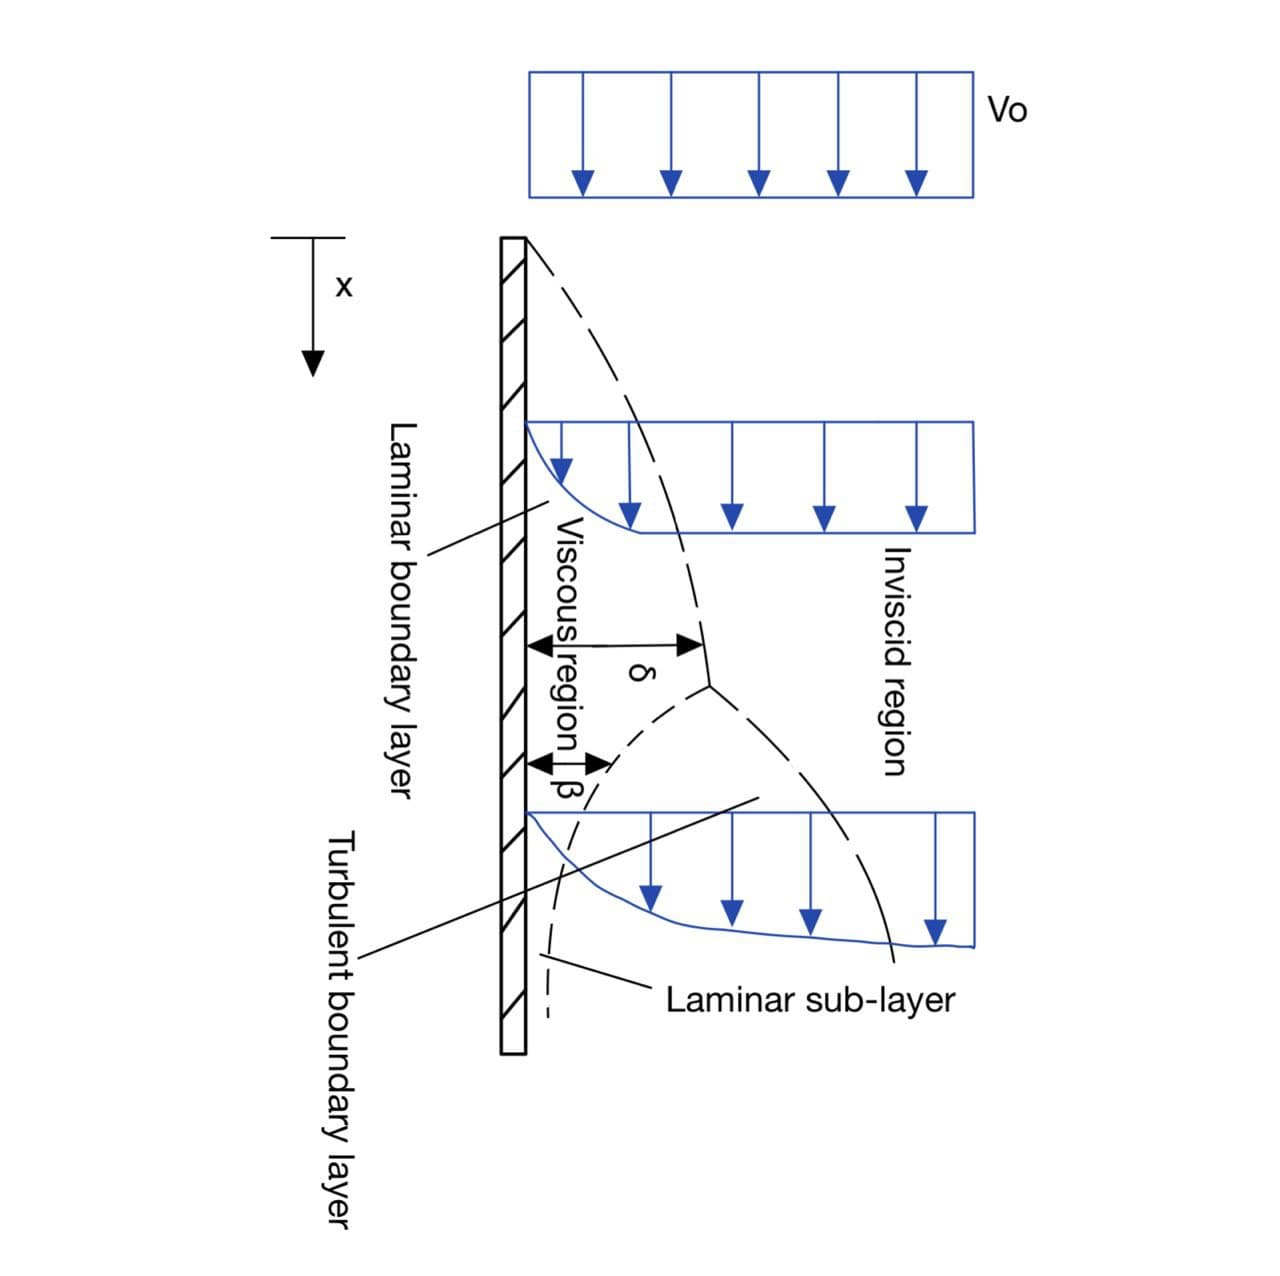
\includegraphics[width=0.65\textwidth]{PICTURES/BL.jpg}
    \caption [Boundary layer formation near a wall] {\textbf{Boundary layer formation near a wall}}
    \label{fig:BL}       % Give a unique label
\end{figure}

According to Prandtl's Boundary layer theory \cite{anderson2005ludwig}, 
\begin{equation}\label{eq:BL}
    \begin{aligned} \delta &\approx \begin{cases}\begin{aligned}
        &\frac{5.0x}{{Re^{1/2}}_x} &\textrm{laminar} \\ \\
        &\frac{0.16x}{{Re^{1/7}}_x} &\textrm{turbulent}\\
    \end{aligned}\end{cases}
\end{aligned}
\end{equation}
Reynolds number for the flow field along the wall:
\begin{equation}
Re_x = \frac{v_0x}{\nu} \\
\end{equation}

Reynolds number for open-channel flow \cite{french1985open}:
\begin{equation}
\begin{aligned} 
        Re_x & < 500 &\textrm{laminar} \\
        Re_x & > 12500 &\textrm{turbulent} \\
    \end{aligned}
\end{equation}

For the velocities 1mm/min, 0.5mm/min and 5mm/min, maximum wall length($x$) of 15mm, and kinematic viscosity($\nu$) of 
water at 10$^\circ$C 1.3063e-6 [$\mathrm{m^2/s}$] \cite{wagner2008iapws} boundary layer thickness was calculated using \Cref{eq:BL}. 
Boundary layer thickness at the end of the wall for flow-velocity 1mm/min was calculated approximately equal to 170mm; 
for flow-velocity 5mm/min, it was 75mm; and for flow-velocity 0.5mm/min, it was 240mm. As discussed in the chapter 
\ref{chapter:numericalmodel}, subsection \ref{ssec:impdum}, we chose small domain as the primary goal of this thesis was to 
implement chemical kinetics of calcite dissolution and its coupling with the freeflow Navier-Stokes model. 
The width of the domain on the x-axis is just 5mm compared to the calculated boundary layer thickness, we were essentially 
inside the viscous region. Hence, we can expect nothing to very small differences in calculating the rate of calcite dissolution and concentration 
of primary variables when varying grid grading near the wall. To verify the model in \DuMuX is 
consistent with the mathematical calculation, we set the grid grading scenarios near the reactive wall as shown in \Cref{fig:BL}. \\

\section{\DuMuX Simulation results}

\subsection{Time series plot: Open system}\label{ssec:timeSeriesOpen}
For an open system in \DuMuX, the model domain of size [5mm $\times$ 15mm] was divided into ten segments along the x-axis and twenty segments along the y-axis. 
\Cref{fig:OpenedSystem} shows the model domain and boundary conditions set in \DuMuX for an open system scenario. 
A cell at the center of the reactive wall was selected to visualize the variation of a few variables (pH, $\mathrm{m^{Ca^{2+}}}$, $\mathrm{m^{TIC}}$, 
$\mathrm{m^{CO_3^{2-}}}$, $\mathrm{r_{diss}}$) in time.  
The calculation of source/sink terms in \DuMuX was invoked only at the reactive wall and for the rest of 
the domain, the governing equations without the source/sink term were solved. \\
Therefore, we chose a cell at the reactive wall to better understand the dissolution
and its dependency with the other variables. It could have been any cell at the wall, the values could also have been averaged over the cells at the wall, but we 
chose a center cell at the reactive wall, which was an arbitrary decision. The decision does not alter the derived conclusions from the plots below; the focus is on 
understanding the dependency rather than calculating a precise value for these variables (pH, $\mathrm{m^{Ca^{2+}}}$, $\mathrm{m^{TIC}}$, 
$\mathrm{m^{CO_3^{2-}}}$, $\mathrm{r_{diss}}$).

\subsubsection*{Different flow velocities}\label{ssec:diffFlowVel}
The flow-velocity/velocity of \ce{CO2} fingers was varied for this scenario. We assumed three different flow-velocities, 1mm/min, 0.5mm/min and 5mm/min, 
for simulation runs. We set the initial pH of the karst water to 6 but did not include a grid grading parameter in the input file. 
We set the initial concentration of TIC throughout the domain to 2.5e-7 [mol\_\ce{TIC}/mol\_\ce{H2O}], an assumed value, and the 
boundary condition at the top of the domain to 9.9956e-4 [mol/mol], a measured value at 8$^{\circ}$C and 1.0 atm pressure for a cave \cite{Class2020}. \\

\begin{figure}[!h]
        \centering
    \begin{subfigure}{.5\linewidth}
        \centering
        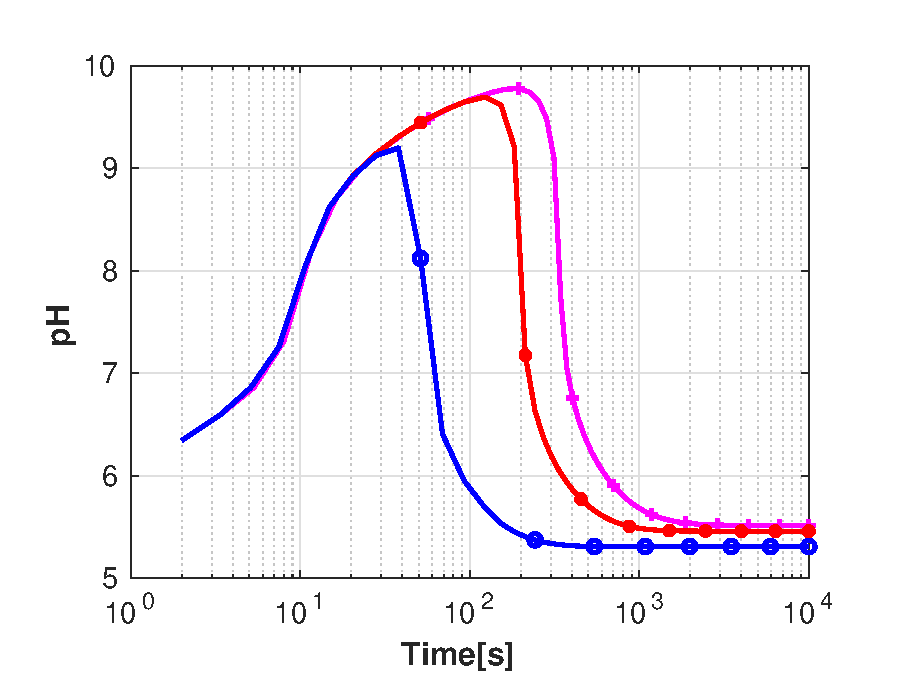
\includegraphics[width=\textwidth]{PICTURES/with_vel_pH.eps}
        \caption{\small Change in pH}
        \label{fig:velpH}       % Give a unique label
    \end{subfigure}%
        \hfill
        % here was an empty line which caused that the plots where not next
        % to each other but on top of each other
    \begin{subfigure}{.5\linewidth}
        \centering
        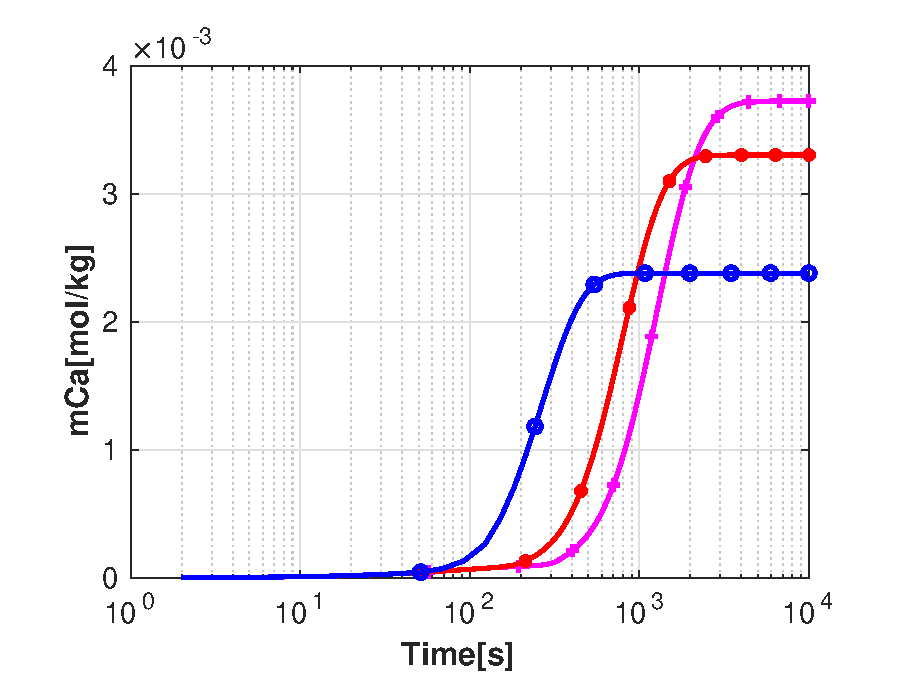
\includegraphics[width=\textwidth]{PICTURES/with_vel_mCa.eps}
        \caption{\small Change in molality of calcium (mCa)}
        \label{fig:velmCa}       % Give a unique label
    \end{subfigure}%
        \hfill
    \begin{subfigure}{.5\linewidth}
        \centering
        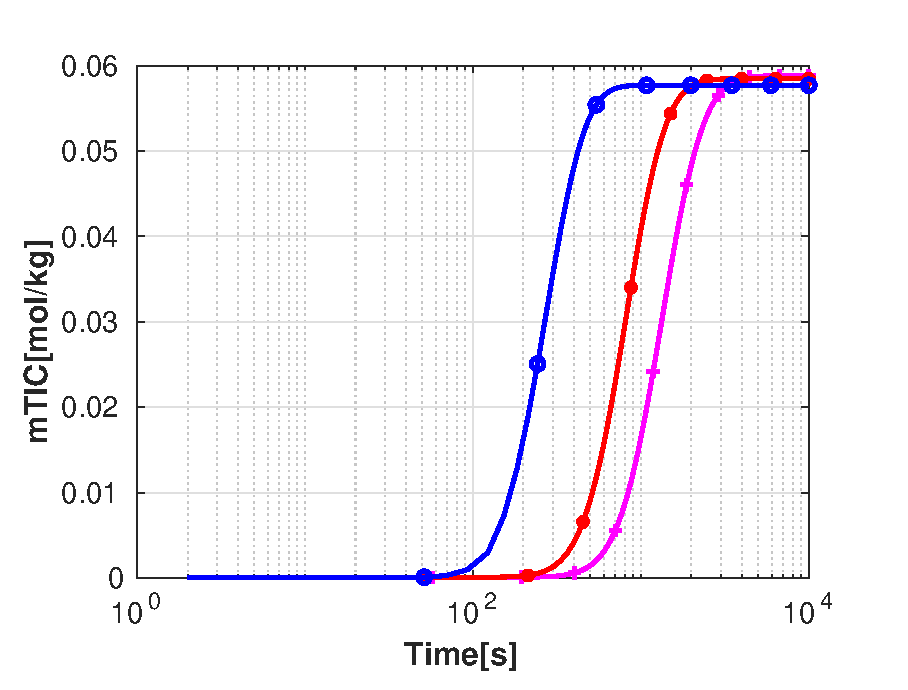
\includegraphics[width=\textwidth]{PICTURES/with_vel_mTIC.eps}
        \caption{\small Change in molality of total inorganic carbon (mTIC)}
        \label{fig:velmTIC}
    \end{subfigure}%
    \hfill
    \begin{subfigure}{.5\linewidth}
        \centering
        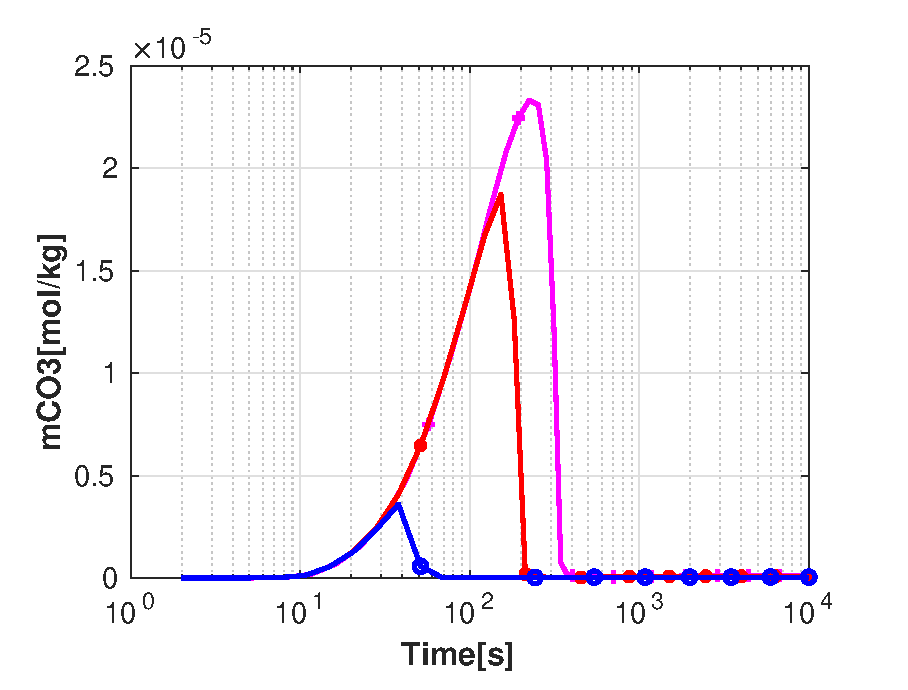
\includegraphics[width=\textwidth]{PICTURES/with_vel_mCO3.eps}
        \caption{\small Change in molality of carbonate (mCO3)}
        \label{fig:velmCO3}
    \end{subfigure}%
    \hfill
    \begin{subfigure}{.5\linewidth}
        \centering
        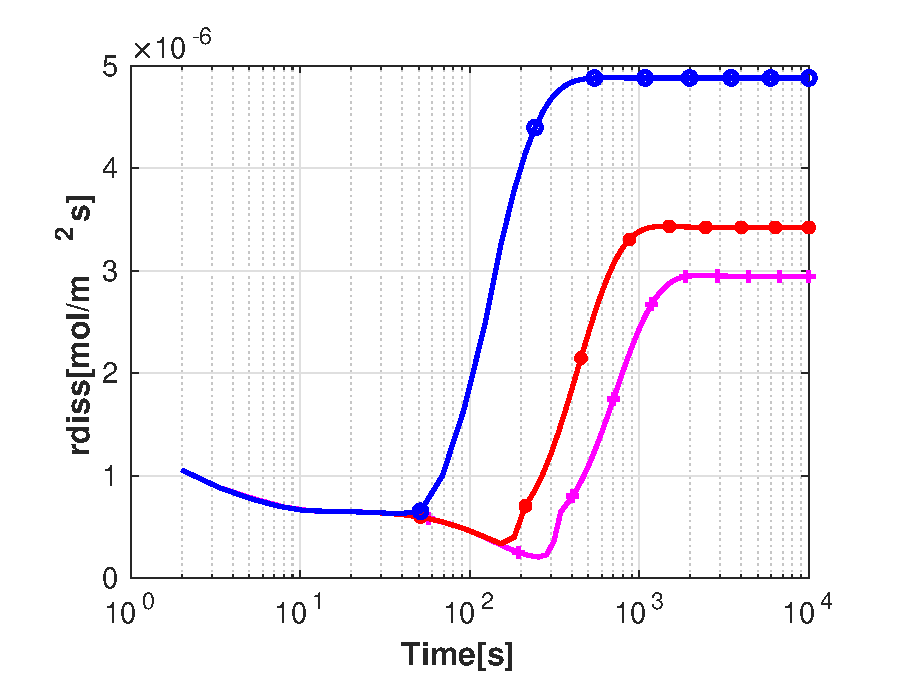
\includegraphics[width=\textwidth]{PICTURES/with_vel_rdiss.eps}
        \caption{\small Change in rate of dissolution of calcite (rdiss)}
        \label{fig:velrdiss}
    \end{subfigure}%
    \begin{subfigure}{.5\linewidth}
        \centering
        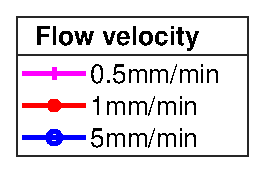
\includegraphics[width=0.40\textwidth]{PICTURES/with_vel_legend.eps}
        \caption{\small Legend}
        \label{fig:vellegend}
    \end{subfigure}%
    \hfill
     \caption [\DuMuX results for different flow velocities in an open system.] {\textbf{\DuMuX results 
     for different flow velocities in an open system.} \small Time series plot for pH (\Cref{fig:velpH}), 
     molality of calcium (\Cref{fig:velmCa}), molality of total inorganic carbon (\Cref{fig:velmTIC}), molality of 
     carbonate (\Cref{fig:velmCO3}) and rate of dissolution of calcite (\Cref{fig:velrdiss}).}
     \label{fig:comparisionDiffFlowVelocity}
\end{figure}

At the beginning of the simulation, the initial concentration of TIC, 2.5e-7 [mol/mol], triggered calcite dissolution. 
As the simulation proceeded, the dissolution potential, determined by the amount of carbonic acid, in the cell at the center of the reactive wall
got depleted which lowered the rate of calcite dissolution as shown in \Cref{fig:velrdiss} and as a consequence increased the pH of the solution as shown in 
\Cref{fig:velpH}. Meanwhile, flow-velocity carried atmospheric \ce{CO2} of concentration 9.9956e-4 [mol/mol], much higher 
than the initial concentration, into the solution. With the new batch of \ce{CO2} coming in, the depleted dissolution potential got recovered. \\

The faster the flow-velocity, the faster the replenishment of the depleted dissolution potential and 
higher the rate of dissolution, as seen in the \Cref{fig:velrdiss}. Flow with higher velocity would bring \ce{CO2} into the solution at a faster rate; 
therefore, the solution would have more carbonic acid which acts as a fuel for dissolution. \Cref{fig:velrdiss} shows flow-velocity with higher value
has a higher rate of dissolution at any given moment in time -- except for the initial few seconds when the rates of dissolution are equal since the 
initial TIC concentration is the only impetus for the calcite dissolution. \\

The faster the flow-velocity, the faster the system reaches steady-state. Steady-state would form an equilibrium between added acidity due to the 
transport of \ce{CO2} into the solution and the resultant alkalinity formed due to calcite dissolution. The higher the flow-velocity, 
the lower is the steady-state pH and higher is the steady-state concentration of calcium as shown in \Cref{fig:velpH,fig:velmCa}.  
At the steady-state, dissociation reactions of calcite (\Cref{eq:CalciteDiss}) shifts more to the right 
forming \ce{Ca^{2+}}, \ce{HCO3^-}, \ce{CO3^{2-}} and \ce{H2O}. 

On the other hand dissociation reactions (\Cref{eq:CarbonicAcidDiss,eq:BicarbonateDiss}) of carbonic acid shift more to the left 
forming carbonic acid and bicarbonate. Therefore, the steady-state concentration of carbonate decays to near zero as shown in \Cref{fig:velmCO3}.


\subsubsection*{Different initial pH} \label{ssec:diffpH}

The initial pH of karst water was varied for this scenario. We assumed four different initial pH, 6, 7, 8, and 9, 
for simulation runs. We set the flow-velocity/velocity of \ce{CO2} fingers to 1mm/min but did not include grid grading 
parameter in the input file. We set the initial concentration of TIC throughout the domain to 2.5e-7 [mol\_\ce{TIC}/mol\_\ce{H2O}], 
an assumed value, and the boundary condition at the top of the domain to 9.9956e-4 [mol/mol], a measured value at 8$^{\circ}$C 
and 1.0 atm pressure for a cave \cite{Class2020}. \\

\begin{figure}[!h]
        \centering
    \begin{subfigure}{.5\linewidth}
            \centering
        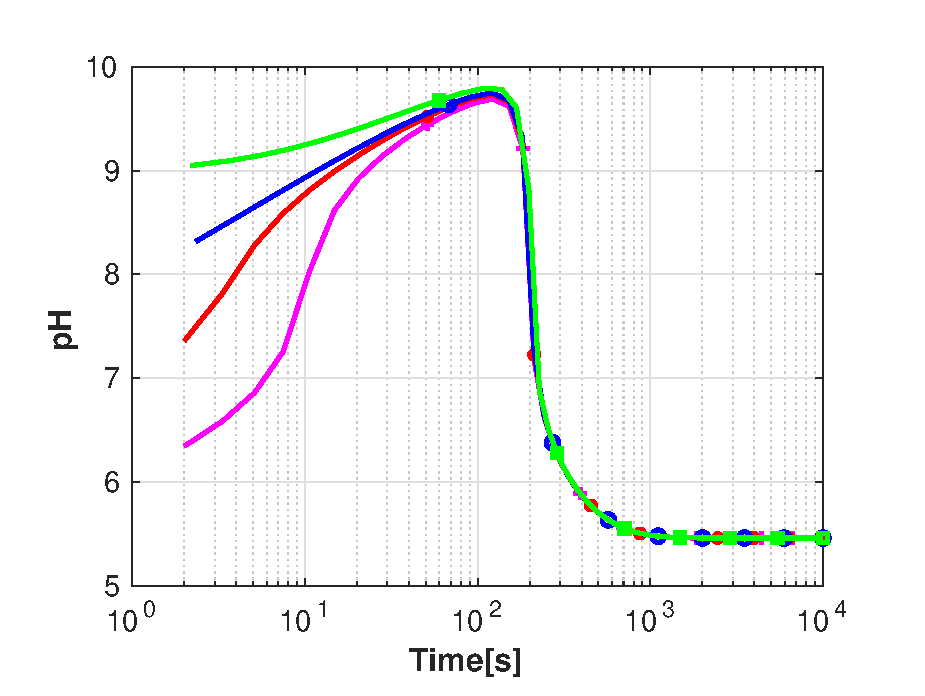
\includegraphics[width=\textwidth]{PICTURES/with_pH_pH.eps}
        \caption{\small Change in pH}
        \label{fig:pHpH}
    \end{subfigure}%
        \hfill
    \begin{subfigure}{.5\linewidth}
            \centering
        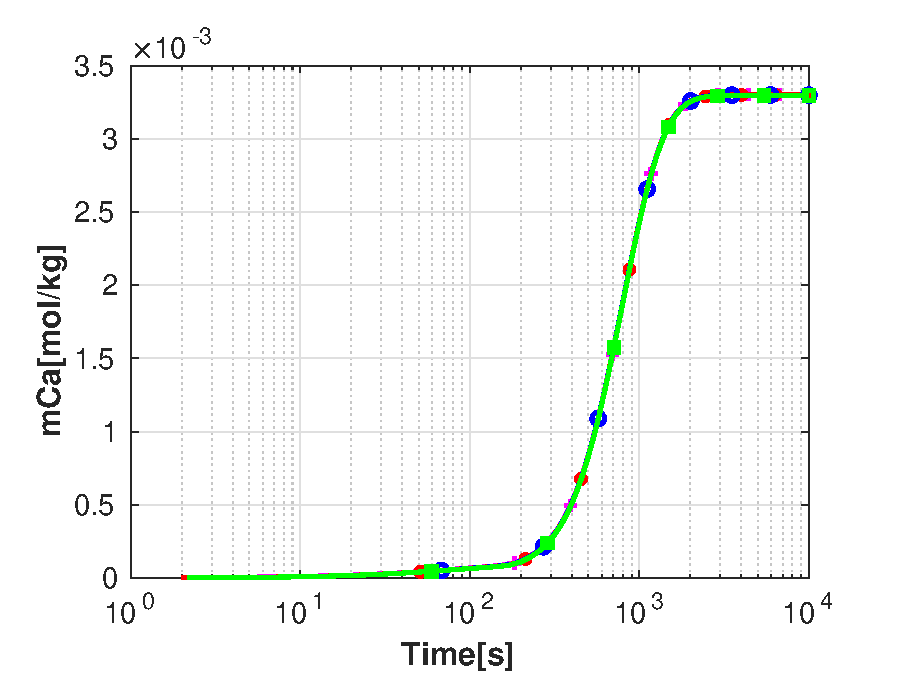
\includegraphics[width=\textwidth]{PICTURES/with_pH_mCa.eps}
        \caption{\small Change in molality of calcium (mCa)}
        \label{fig:pHmCa}
    \end{subfigure}%
    \hfill
    \begin{subfigure}{.5\linewidth}
            \centering
        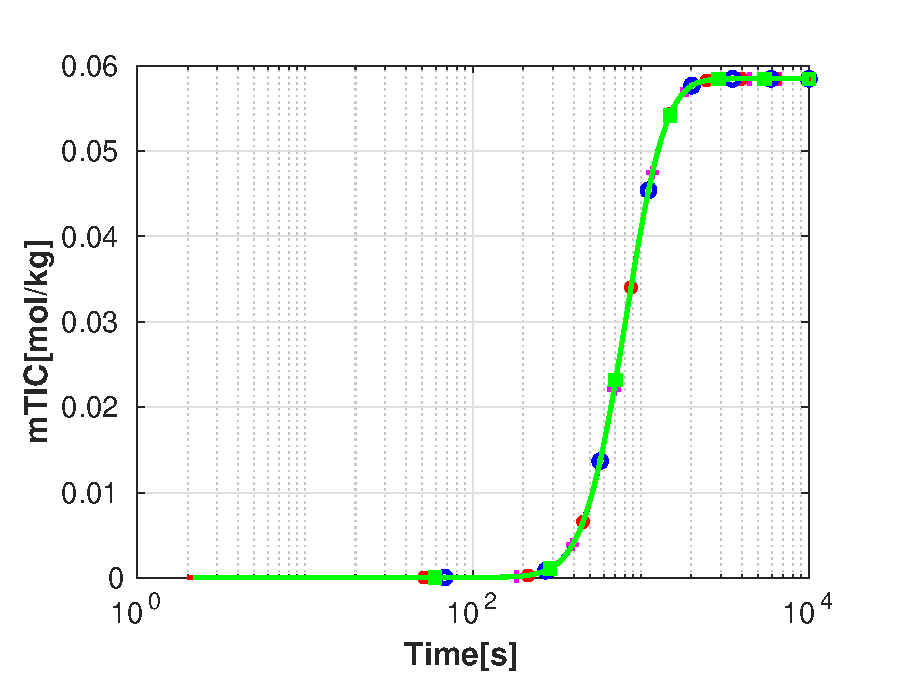
\includegraphics[width=\textwidth]{PICTURES/with_pH_mTIC.eps}
        \caption{\small Change in molality of total inorganic carbon (mTIC)}
        \label{fig:pHmTIC}
    \end{subfigure}%
    \hfill
    \begin{subfigure}{.5\linewidth}
            \centering
        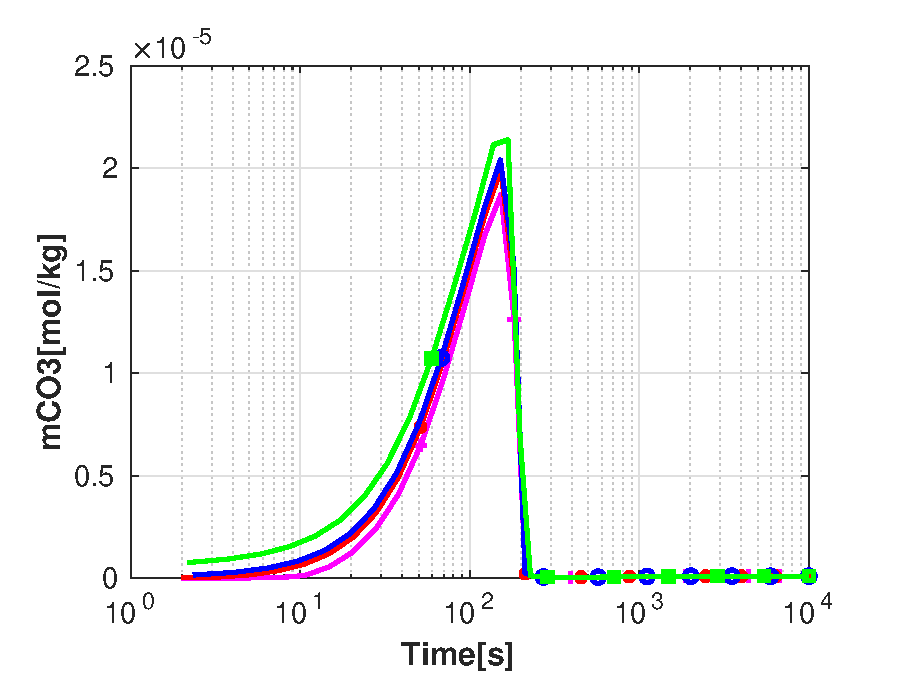
\includegraphics[width=\textwidth]{PICTURES/with_pH_mCO3.eps}
        \caption{\small Change in molality of carbonate (mCO3)}
        \label{fig:pHmCO3}
    \end{subfigure}%
    \hfill
    \begin{subfigure}{.5\linewidth}
            \centering
        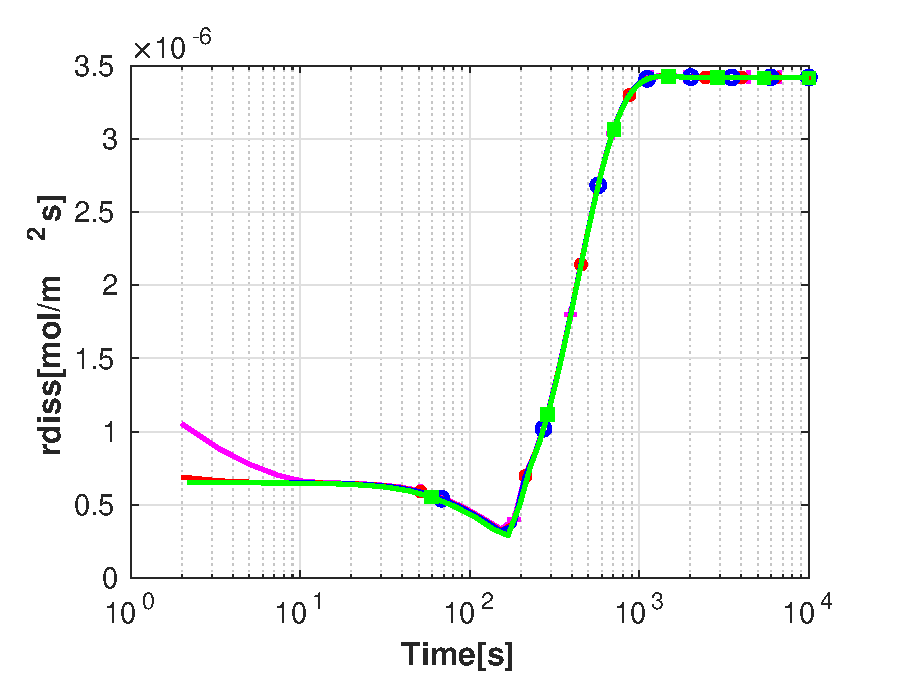
\includegraphics[width=\textwidth]{PICTURES/with_pH_rdiss.eps}
        \caption{\small Change in rate of dissolution of calcite (rdiss)}
        \label{fig:pHrdiss}
    \end{subfigure}%
  \hfill
  \begin{subfigure}{.5\linewidth}
            \centering
        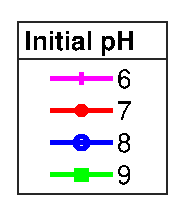
\includegraphics[width=0.25\textwidth]{PICTURES/with_pH_legend.eps}
        \caption{\small Legend}
        \label{fig:pHlegend}
    \end{subfigure}%
    \caption [\DuMuX results for different initial pH in an open system.] {\textbf{\DuMuX results for different initial pH in an open system.} 
    \small Time series plot for pH (\Cref{fig:pHpH}), molality of calcium (\Cref{fig:pHmCa}), 
    molality of total inorganic carbon (\Cref{fig:pHmTIC}), molality of carbonate (\Cref{fig:pHmCO3}) and rate of 
    dissolution of calcite (\Cref{fig:pHrdiss}).}
    \label{fig:comparisionDiffInitialpH}
\end{figure} 


Unlike the scenario with different flow-velocity, it is safe to say that the rate of calcite dissolution and concentration of primary variables 
does not depend on the initial pH. 
Since we had different initial pH of the karst water, the pH and rate of dissolution plots (\Cref{fig:pHpH,fig:pHrdiss}) look out of sync at the beginning but quickly adapts to identical values. 
As we saw in \Cref{ssec:diffFlowVel}, the rate of calcite dissolution is strongly dependent on the flow-velocity and TIC concentration in the solution. 
Since these values (flow-velocity and TIC concentration in the solution) were constant in this scenario we did not see much differences in the plots. Initial 
inconsistency in the rate of dissolution and concentrations is because of the difference in the initial concentration of hydrogen which is used, together with TIC, 
to calculate carbonate and bicarbonate concentrations. 


\subsubsection*{Different boundary \ce{CO2} concentrations} \label{ssec:diffInitialBC}
The \ce{CO2} concentration at the top boundary was varied for this scenario. We assumed three different \ce{CO2} concentrations, 
1.5993e-6, 9.9956e-4, and 9.9956e-2 [mol/mol], for simulation runs. We set the flow-velocity/velocity of \ce{CO2} fingers to 1mm/min 
and initial pH to 6 but did not include grid grading parameter in the input file. We set the initial concentration of 
TIC throughout the domain to 2.5e-7 [mol\_\ce{TIC}/mol\_\ce{H2O}], which was an assumed value. \\

\begin{figure}[!h]
        \centering
    \begin{subfigure}{.5\linewidth}
            \centering
        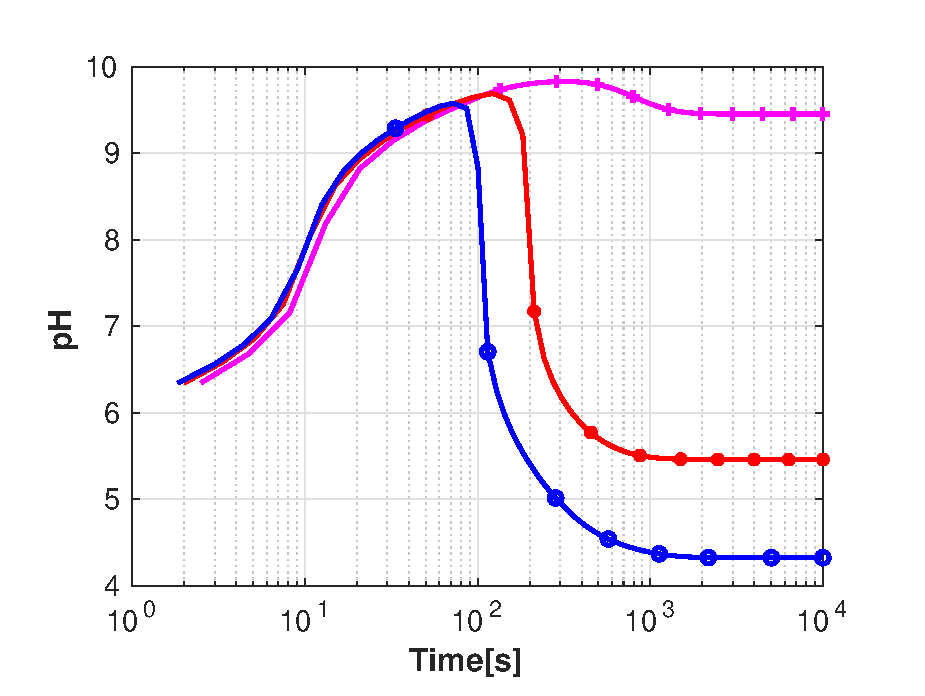
\includegraphics[width=\textwidth]{PICTURES/with_CO2_pH.eps}
        \caption{\small Change in pH}
        \label{fig:CO2pH}
    \end{subfigure}%
        \hfill
    \begin{subfigure}{.5\linewidth}
            \centering
        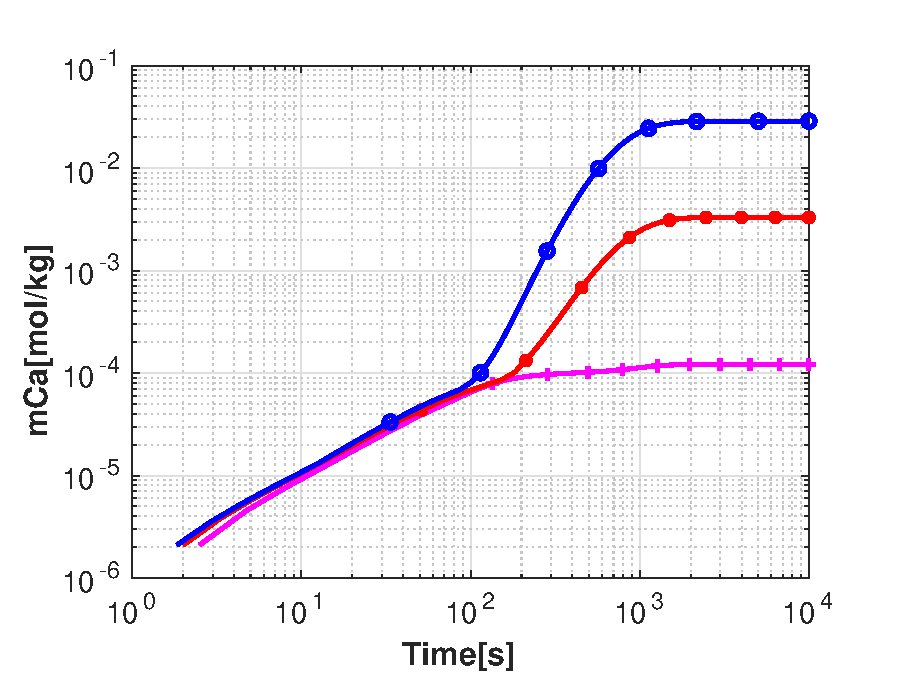
\includegraphics[width=\textwidth]{PICTURES/with_CO2_mCa.eps}
        \caption{\small Change in molality of calcium (mCa)}
        \label{fig:CO2mCa}
    \end{subfigure}%
        \hfill
    \begin{subfigure}{.5\linewidth}
            \centering
        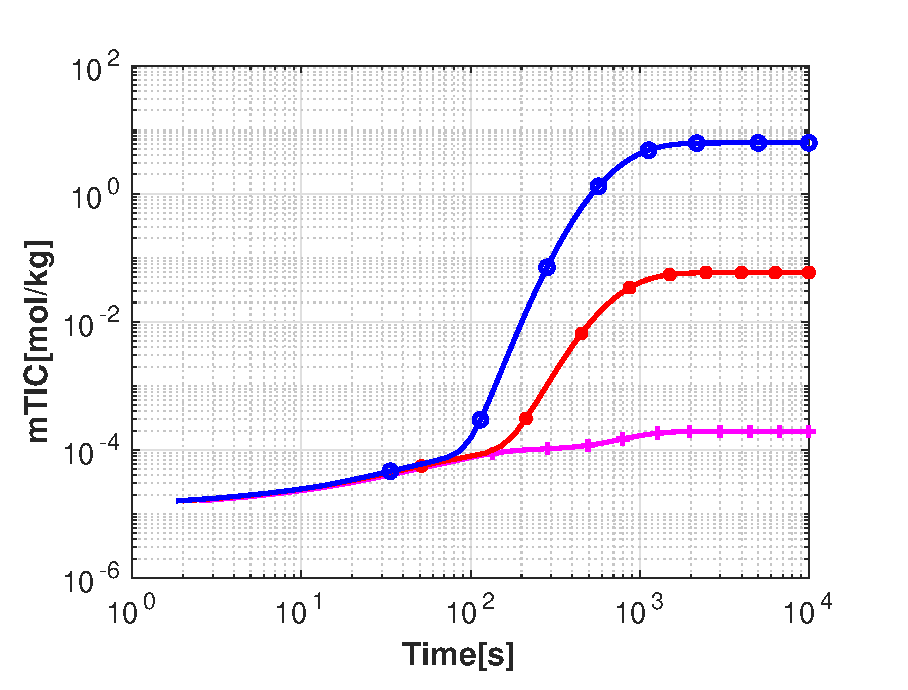
\includegraphics[width=\textwidth]{PICTURES/with_CO2_mTIC.eps}
        \caption{Change in molality of total inorganic carbon (mTIC)}
        \label{fig:CO2mTIC}
    \end{subfigure}%
    \hfill
    \begin{subfigure}{.5\linewidth}
            \centering
        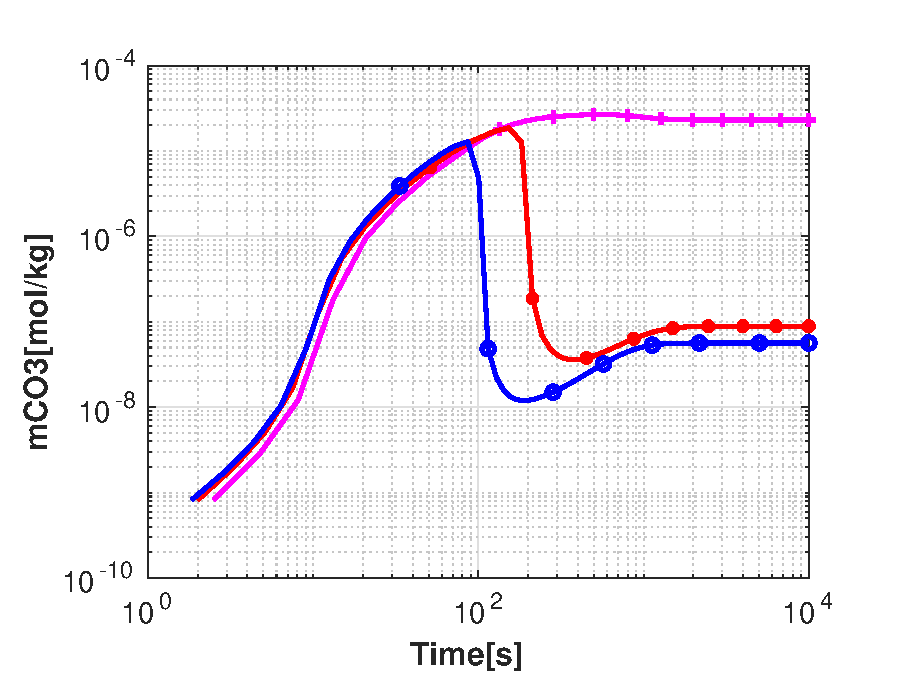
\includegraphics[width=\textwidth]{PICTURES/with_CO2_mCO3.eps}
        \caption{\small Change in molality of carbonate (mCO3)}
        \label{fig:CO2mCO3}
    \end{subfigure}%
    \hfill
    \begin{subfigure}{.5\linewidth}
            \centering
        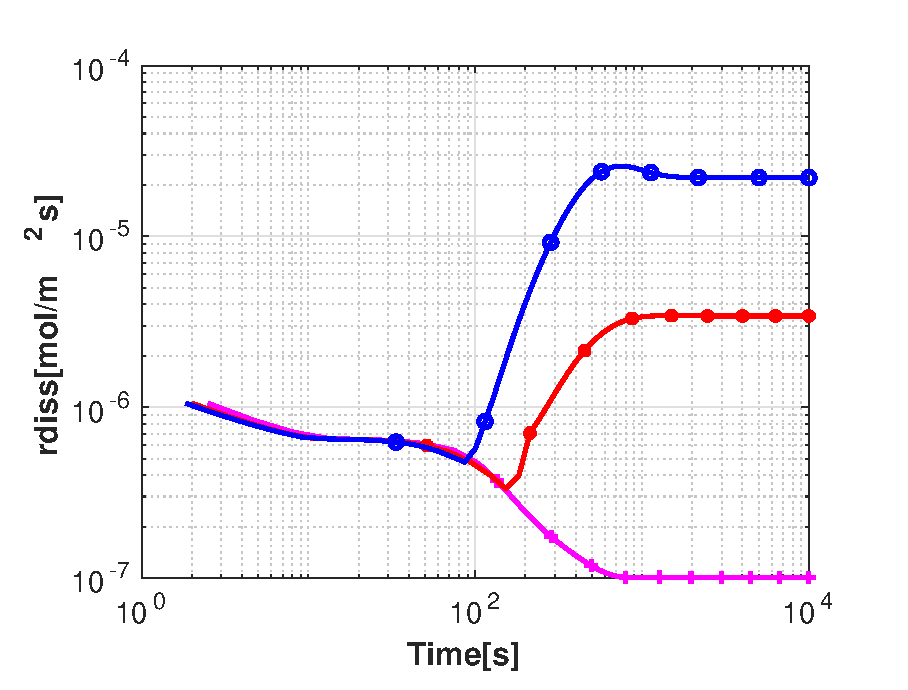
\includegraphics[width=\textwidth]{PICTURES/with_CO2_rdiss.eps}
        \caption{\small Change in rate of dissolution of calcite (rdiss)}
        \label{fig:CO2rdiss}
    \end{subfigure}%
    \hfill
    \begin{subfigure}{.5\linewidth}
            \centering
        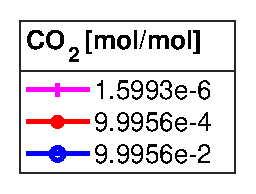
\includegraphics[width=0.35\textwidth]{PICTURES/with_CO2_legend.eps}
        \caption{\small Legend}
        \label{fig:CO2legend}
    \end{subfigure}%
    \caption [\DuMuX results for different \ce{CO2} concentration at the top of the domain in an open system.] {\textbf{\DuMuX results for different \ce{CO2} 
    concentration at the top of the domain in an open system.} \small Time series plot for 
    pH (\Cref{fig:CO2pH}), molality of calcium (\Cref{fig:CO2mCa}), molality of total inorganic carbon (\Cref{fig:CO2mTIC}), 
    molality of carbonate (\Cref{fig:CO2mCO3}) and rate of 
    dissolution of calcite (\Cref{fig:CO2rdiss}).}
    \label{fig:diffCO2}
\end{figure}

Similar to the scenario in \Cref{ssec:diffFlowVel} the initial concentration of TIC, 2.5e-7 [mol/mol], triggered calcite dissolution. 
But unlike the scenario in \Cref{ssec:diffFlowVel}, now the flow-velocity entering the domain carries different concentrations of \ce{CO2}. 
The higher the concentration of \ce{CO2} in the incoming water, the higher is the elevation of dissolution potential of the karst water and, consequently, higher is 
the calcite dissolution and concentration of TIC, as shown in \Cref{fig:CO2rdiss,fig:CO2mCa,fig:CO2mTIC}. \\

The higher concentration of \ce{CO2} in the incoming water produces a higher concentration of carbonic acid which decreases the pH of 
the solution (\Cref{fig:CO2pH}). The rate of calcite dissolution decreases for the \ce{CO2} concentration
of 1.5993e-6 [mol/mol] as it reaches the steady-state which shifts the dissociation reactions of calcite more to the left. 
On the other hand dissociation reactions of carbonic acid shift more to the right forming carbonate and bicarbonate. 
\Cref{fig:CO2mCO3} illustrates the concentration of carbonate higher for the lowest among the other two concentrations of \ce{CO2}.


\subsubsection*{Different Grid grading parameter} \label{ssec:diffGrid}

The grid grading parameter was varied for this scenario. We assumed three different grid grading values, 
1.0 (without grid grading), 1.1 and 1.2, for simulation runs. We set the flow-velocity/velocity of \ce{CO2} fingers to 1mm/min 
and initial pH to 6. We set the initial concentration of TIC throughout the domain to 2.5e-7 [mol\_\ce{TIC}/mol\_\ce{H2O}], 
an assumed value, and the boundary condition at the top of the domain to 9.9956e-4 [mol/mol], a measured value at 8$^{\circ}$C 
and 1.0 atm pressure for a cave \cite{Class2020}. \\

\Cref{fig:diffGrid} helps in comparing the numerical model with the mathematical model presented in \Cref{para:definitionGridGrading}
for the resolution of a boundary layer near the wall. \\

\begin{figure}[!h]
        \centering
    \begin{subfigure}{.5\linewidth}
            \centering
        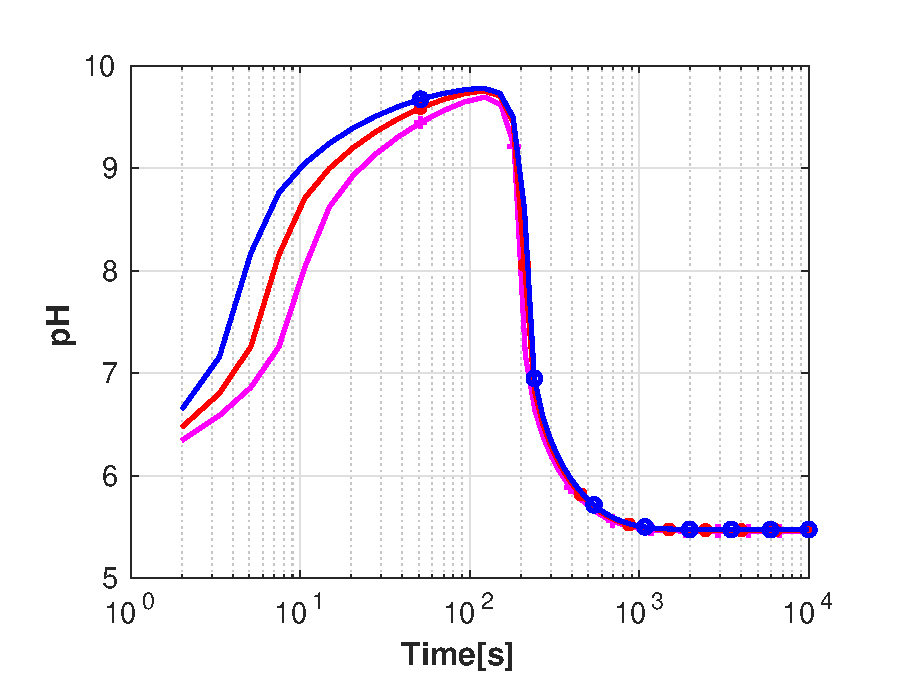
\includegraphics[width=\textwidth]{PICTURES/with_grid_pH.eps}
        \caption{\small Change in pH}
        \label{fig:gridpH}
    \end{subfigure}%
        \hfill
    \begin{subfigure}{.5\linewidth}
            \centering
        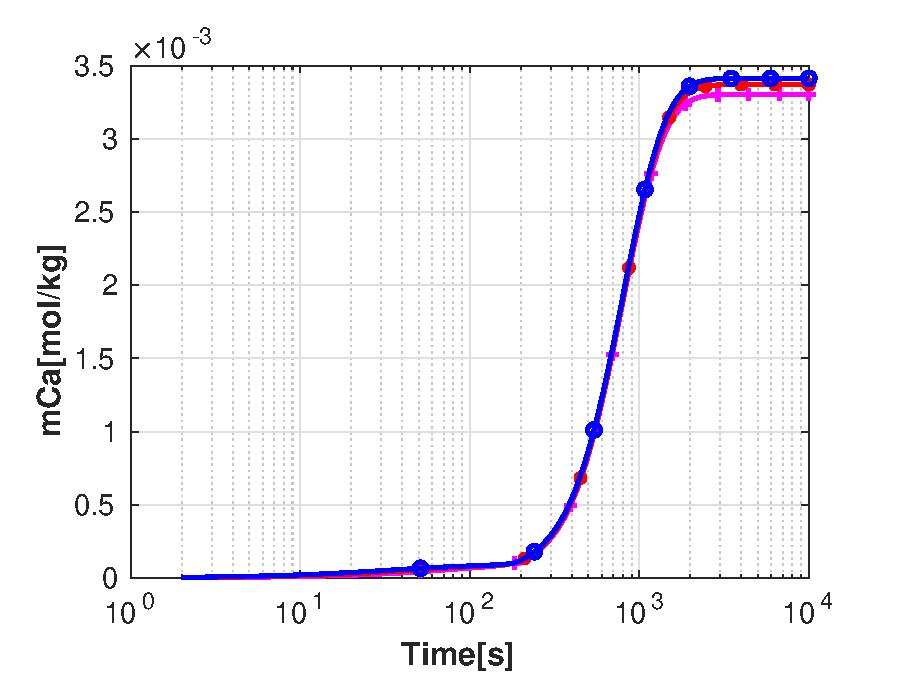
\includegraphics[width=\textwidth]{PICTURES/with_grid_mCa.eps}
        \caption{\small Change in molality of calcium (mCa)}
        \label{fig:gridmCa}
    \end{subfigure}%
        \hfill
        \begin{subfigure}{.5\linewidth}
            \centering
        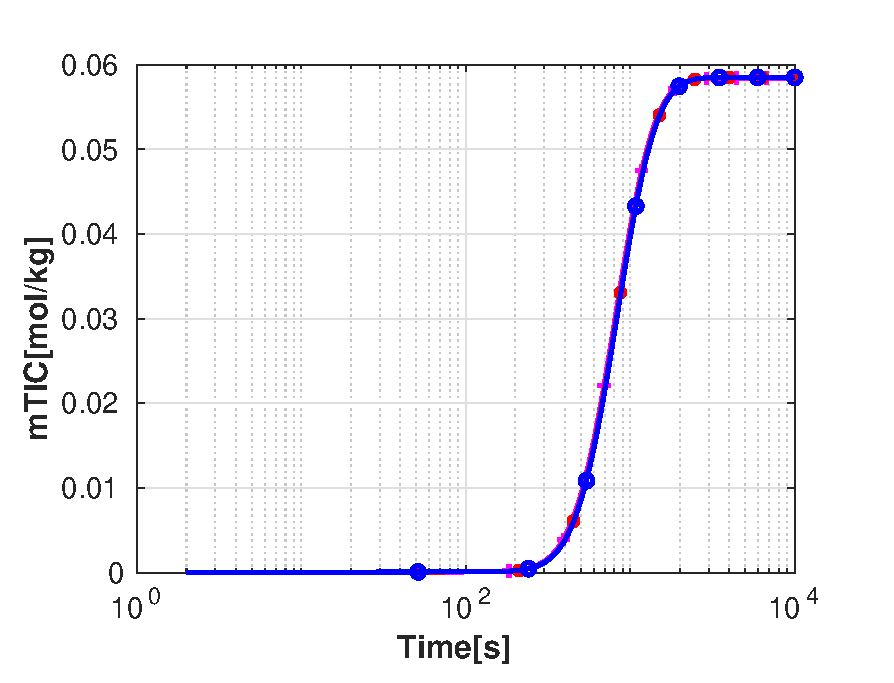
\includegraphics[width=\textwidth]{PICTURES/with_grid_mTIC.eps}
        \caption{\small Change in molality of total inorganic carbon (mTIC)}
        \label{fig:gridmTIC}
    \end{subfigure}%
        \hfill
        \begin{subfigure}{.5\linewidth}
            \centering
        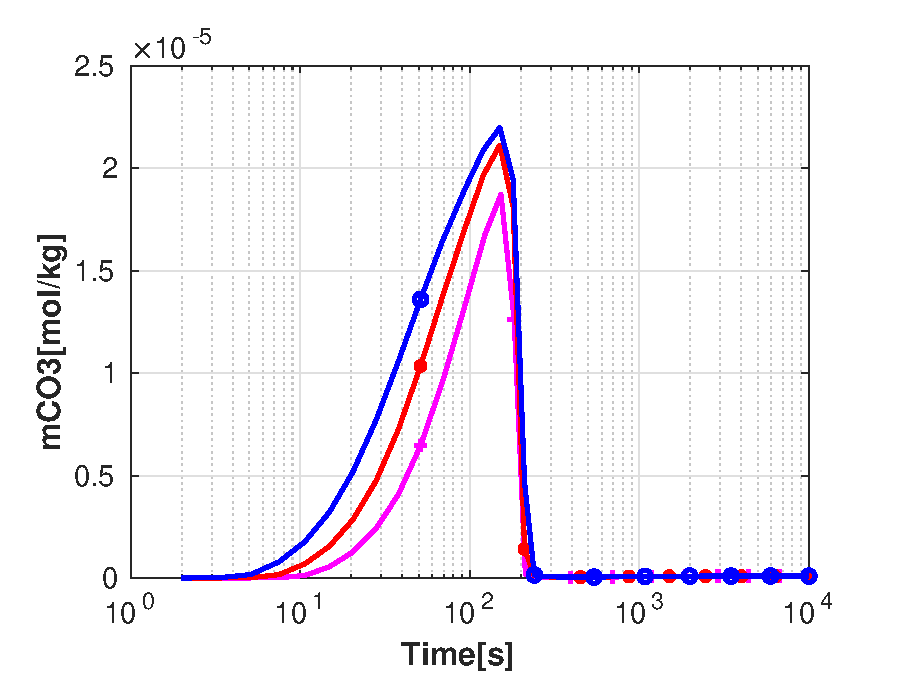
\includegraphics[width=\textwidth]{PICTURES/with_grid_mCO3.eps}
        \caption{\small Change in molality of carbonate (mCO3)}
        \label{fig:gridmCO3}
    \end{subfigure}%
        \hfill
        \begin{subfigure}{.5\linewidth}
            \centering
        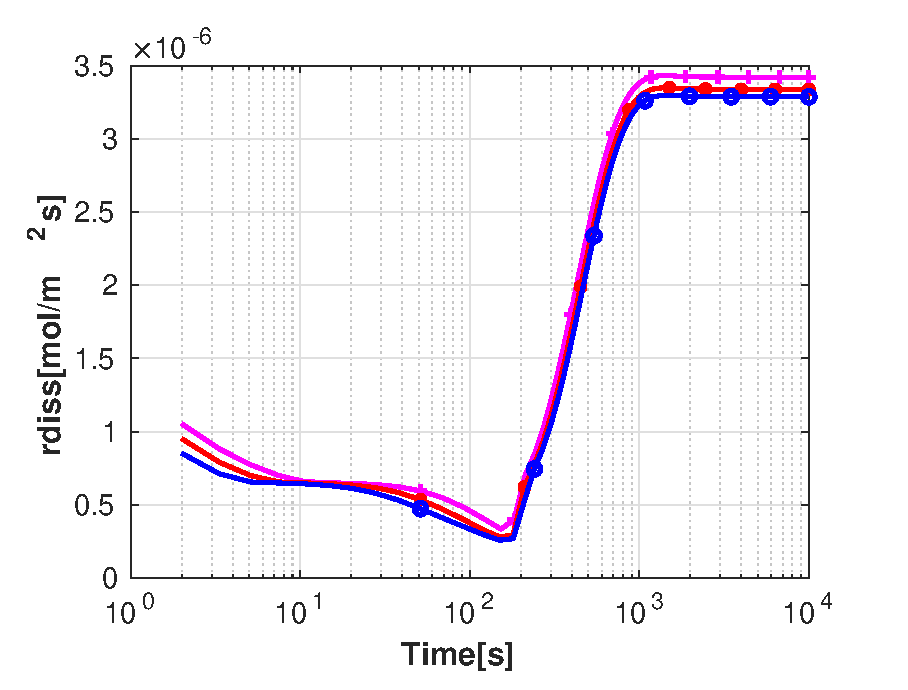
\includegraphics[width=\textwidth]{PICTURES/with_grid_rdiss.eps}
        \caption{\small Change in rate of dissolution of calcite (rdiss)}
        \label{fig:gridrdiss}
    \end{subfigure}%
        \hfill
        \begin{subfigure}{.5\linewidth}
            \centering
        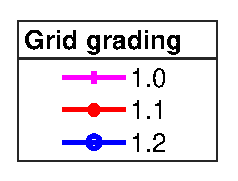
\includegraphics[width=0.35\textwidth]{PICTURES/with_grid_legend.eps}
        \caption{\small Legend}
        \label{fig:gridlegend}
    \end{subfigure}%
    \caption [\DuMuX results for different grid grading parameter in an open system.] {\textbf{\DuMuX results for 
    different grid grading parameter in an open system.} \small Time series plot for pH (\Cref{fig:gridpH}), 
    molality of calcium (\Cref{fig:gridmCa}), 
    molality of total inorganic carbon (\Cref{fig:gridmTIC}), molality of carbonate (\Cref{fig:gridmCO3}) 
    and rate of dissolution of calcite (\Cref{fig:gridrdiss}).}
    \label{fig:diffGrid}
\end{figure}

\Cref{fig:diffGrid} confirms with the mathematical calculation we had for our model that there are only minor differences 
in calculating the rate of calcite dissolution and concentration of primary variables when varying grid grading near the wall. 
The plots are a little out of sync at the beginning of the simulation. A higher grid grading would mean a smaller domain size near 
the reactive wall. Therefore, a smaller domain would have a faster depletion of carbonic acid and a faster rise in pH as shown in \Cref{fig:gridpH} but 
as soon as the depleted potential gets replenished by the incoming \ce{CO2} transported with the flow, pH along with the rate of dissolution and concentration of 
$\mathrm{m^{Ca^{2+}}}$, $\mathrm{m^{TIC}}$ and $\mathrm{m^{CO_3^{2-}}}$ adapts to identical values. 

\subsection{Contour plots: Open System} \label{ssec:contour}
For an open system in \DuMuX, steady-state contour plots for a model domain of size [5mm $\times$ 15mm] are presented and explained in this subsection.
The model domain has, as in \ref{ssec:timeSeriesOpen}, ten segments along the x-axis and twenty segments along the y-axis. We saw in \ref{ssec:diffFlowVel}
the rate of calcite dissolution and concentrations of primary variables depend strongly on flow-velocity and the boundary/initial \ce{CO2} concentration. 
The flow-velocity/velocity of \ce{CO2} fingers was varied for this scenario. \\
We set the initial pH of the karst water to 6 and set the grid grading to 1.1 in the input file. 
We set the initial concentration of TIC throughout the domain to 2.5e-7 [mol\_\ce{TIC}/mol\_\ce{H2O}], an assumed value, and the 
boundary condition at the top of the domain to 9.9956e-4 [mol/mol], a measured value at 8$^{\circ}$C and 1.0 atm pressure for a cave \cite{Class2020}. \\
We assumed three different flow-velocities, 1mm/min, 0.5mm/min and 5mm/min, for simulation runs to understand the steady-state spatial distribution of 
pH, $\mathrm{m^{Ca^{2+}}}$, $\mathrm{m^{TIC}}$ and $\mathrm{m^{CO_3^{2-}}}$. 
All the plots in this subsection were obtained from Paraview \cite{ahrens2005paraview}.

\subsubsection*{pH contour plots} \label{sssec:contourpH}

% steady state pH
\begin{figure}[!h]
\centering
    \begin{subfigure}{.5\linewidth}
        \centering
        \includegraphics[trim=500 20 450 20, clip, width=0.9\textwidth]{PICTURES/contour_vel1mm_pH.eps}
        \caption{\small Flow Velocity = 1mm/min}
        \label{fig:pHSteady-state}       % Give a unique label
    \end{subfigure}%
    \hfill
    \begin{subfigure}{.5\linewidth}
        \centering
        \includegraphics[trim=500 20 420 20, clip, width=0.9\textwidth]{PICTURES/contour_vel5mm_pH.eps}
        \caption{\small Flow Velocity = 5mm/min}
        \label{fig:pHSteady-state5mm}       % Give a unique label
    \end{subfigure}%
    \hfill
    \begin{subfigure}{.5\linewidth}
        \centering
        \includegraphics[trim=500 20 450 20, clip, width=\textwidth]{PICTURES/contour_vel0.5mm_pH.eps}
        \caption{\small Flow Velocity = 0.5mm/min}
        \label{fig:pHSteady-state0.5mm}       % Give a unique label
    \end{subfigure}%
    \caption [\DuMuX Contour plots: Numerical results that show the spatial distribution of pH at the steady-state in an open system] {\textbf{\DuMuX Contour plots: Numerical results that show the spatial distribution of pH at the steady-state in an open system}}
     \label{fig:contourpH}
\end{figure}

All the \Cref{fig:pHSteady-state,fig:pHSteady-state5mm,fig:pHSteady-state0.5mm} show higher pH near the reactive wall 
where carbonic acid is used up in calcite dissolution to form carbonate, bicarbonate, and calcium. 
As we go away from the wall, pH decreases gradually as the concentration of carbonic acid in the solution increases . 
The steady-state pH is a composite of carbonic acid and carbonate, bicarbonate, and calcium. Carbonic acid depends on the amount of \ce{CO2} 
transported into the karst water, so, without calcite dissolution, there would be no spatial variation of pH rather some value less than 6. 
On the one hand the products from calcite dissolution (carbonate, bicarbonate, and calcium) slowly get diffused into the system which 
increases the pH but on the other hand the products also get carried 
out of the system with the flow-velocity which would again increase the pH. The farther we go from the wall, the less pronounced is the diffusion 
and ultimately after some distance, the flow-velocity wins over diffusion. \\

A higher flow-velocity means diffusion of carbonate, bicarbonate, and calcium into the system is suppressed; hence, much of the domain would be 
just carbonic acid, as shown in \Cref{fig:pHSteady-state5mm}. 

\subsubsection*{\ce{m^{\ce{CO3^{2-}}}} contour plots} \label{sssec:contourmCO3}

%steady-state CO3
\begin{figure}[!h]
\centering
    \begin{subfigure}{.5\linewidth}
        \centering
        \includegraphics[trim=500 20 450 20, clip, width=0.9\textwidth]{PICTURES/contour_vel1mm_mCO3.eps}
        \caption{\small Flow Velocity = 1mm/min}
        \label{fig:CO3Steady-state}       % Give a unique label
    \end{subfigure}%
    \hfill
    \begin{subfigure}{.5\linewidth}
        \centering
        \includegraphics[trim=500 20 450 20, clip, width=0.9\textwidth]{PICTURES/contour_vel5mm_mCO3.eps}
        \caption{\small Flow Velocity = 5mm/min}
        \label{fig:CO3Steady-state5mm}       % Give a unique label
    \end{subfigure}%
    \hfill
    \begin{subfigure}{.5\linewidth}
        \centering
        \includegraphics[trim=500 20 450 20, clip, width=0.9\textwidth]{PICTURES/contour_vel0.5mm_mCO3.eps}
        \caption{\small Flow Velocity = 0.5mm/min}
        \label{fig:CO3Steady-state0.5mm}       % Give a unique label
    \end{subfigure}%
    \caption [\DuMuX Contour plots: Numerical results that show the spatial distribution of molality of carbonate at the steady-state in an open system] {\textbf{\DuMuX Contour plots: Numerical results that show the spatial distribution of molality of carbonate at the steady-state in an open system}}
     \label{fig:contourCO3}
\end{figure}

Similar to \Cref{fig:contourpH}, all the \Cref{fig:CO3Steady-state,fig:CO3Steady-state5mm,fig:CO3Steady-state0.5mm} show higher 
carbonate concentration near the reactive wall where carbonic acid is used up in calcite dissolution to form carbonate, bicarbonate, and calcium. 
As described in \Cref{sssec:contourpH}, the spatial distribution is a resultant of flow-velocity with which \ce{CO2} is transported into the system, which 
also dictates calcite dissolution, and diffusion of the products formed during dissolution. 

\subsubsection*{\ce{m^{TIC}} contour plots} \label{sssec:contourmTIC}
% steady state TIC
\begin{figure}[!h]
\centering
    \begin{subfigure}{.5\linewidth}
        \centering
        \includegraphics[trim=480 10 450 10, clip, width=0.9\textwidth]{PICTURES/contour_vel1mm_mTIC.eps}
        \caption{\small Flow Velocity = 1mm/min}
        \label{fig:TICSteady-state}       % Give a unique label
    \end{subfigure}%
    \hfill
    \begin{subfigure}{.5\linewidth}
        \centering
        \includegraphics[trim=500 20 450 20, clip, width=0.9\textwidth]{PICTURES/contour_vel5mm_mTIC.eps}
        \caption{\small Flow Velocity = 5mm/min}
        \label{fig:TICSteady-state5mm}       % Give a unique label
    \end{subfigure}%
    \hfill
    \begin{subfigure}{.5\linewidth}
        \centering
        \includegraphics[trim=500 20 450 20, clip, width=0.9\textwidth]{PICTURES/contour_vel0.5mm_mTIC.eps}
        \caption{\small Flow Velocity = 0.5mm/min}
        \label{fig:TICSteady-state0.5mm}       % Give a unique label
    \end{subfigure}%
    \caption [\DuMuX Contour plots: Numerical results that show the spatial distribution of molality of total 
    inorganic carbon at the steady-state in an open system] {\textbf{\DuMuX Contour plots: Numerical results that show the spatial distribution of molality of total 
    inorganic carbon at the steady-state in an open system}}
     \label{fig:contourTIC}
\end{figure}

Total inorganic carbon comprises of \ce{CO2}, \ce{H2CO3}, \ce{CO3^{2-}} and \ce{HCO3^-}. As we described in previous subsections, 
carbonic acid dissolves calcite forming carbonate, bicarbonate, and calcium into the solution. Concentrations of carbonate, bicarbonate, and calcium 
gradually decrease as we go away from the wall and, consequently, the concentration of carbonic acid (\ce{H2CO3}) gradually increases. 
In all of these concentrations (carbonate, bicarbonate, and carbonic acid) change, the total inorganic carbon remains constant, as shown in \Cref{fig:contourTIC}.
The spatial distribution of total inorganic carbon in steady-state does not depend on the flow-velocity. 

\subsubsection*{\ce{m^{\ce{Ca^{2+}}}} contour plots} \label{sssec:contourmCa}

% steady state Ca
\begin{figure}[!h]
\centering
    \begin{subfigure}{.5\linewidth}
        \centering
        \includegraphics[trim=480 10 450 10, clip, width=0.9\textwidth]{PICTURES/contour_vel1mm_mCa.eps}
        \caption{\small Flow Velocity = 1mm/min}
        \label{fig:CaSteady-state}       % Give a unique label
    \end{subfigure}%
    \hfill
    \begin{subfigure}{.5\linewidth}
        \centering
        \includegraphics[trim=500 20 450 20, clip, width=0.9\textwidth]{PICTURES/contour_vel5mm_mCa.eps}
        \caption{\small Flow Velocity = 5mm/min}
        \label{fig:CaSteady-state5mm}       % Give a unique label
    \end{subfigure}%
    \hfill
    \begin{subfigure}{.5\linewidth}
        \centering
        \includegraphics[trim=500 20 450 20, clip, width=0.9\textwidth]{PICTURES/contour_vel0.5mm_mCa.eps}
        \caption{\small Flow Velocity = 0.5mm/min}
        \label{fig:CaSteady-state0.5mm}       % Give a unique label
    \end{subfigure}%
    \caption [\DuMuX Contour plots: Numerical results that show the spatial distribution of molality of calcium at the steady-state in an open system] {\textbf{\DuMuX Contour plots: Numerical results that show the spatial distribution of molality of calcium at the steady-state in an open system}}
     \label{fig:contourCa}
\end{figure}

Similar to \Cref{fig:contourpH,fig:contourCO3}, all the \Cref{fig:CaSteady-state,fig:CaSteady-state5mm,fig:CaSteady-state0.5mm} show higher 
calcium concentration near the reactive wall where carbonic acid is used up in calcite dissolution to form carbonate, bicarbonate, and calcium. 
The explanation to the spatial distribution is exactly the same as described in \Cref{sssec:contourpH,sssec:contourmCO3}.


\subsection{Time series plot: Closed system} \label{ssec:timeSeriesClosed}
For a closed system in \DuMuX a model domain of size [5mm $\times$ 15mm] was divided into ten segments along the x-axis and twenty segments along the y-axis.
A cell at the center of the reactive wall was selected to visualize the variation of a few variables (pH, $\mathrm{m^{Ca^{2+}}}$, $\mathrm{m^{TIC}}$, 
$\mathrm{m^{CO_3^{2-}}}$, $\mathrm{r_{diss}}$) in time, similar to the setup described in \Cref{ssec:timeSeriesOpen}.

\subsubsection*{Different initial pH} \label{ssec:diffinitialpHnoflow}
The initial pH of karst water was varied for this scenario. We assumed four different initial pH, 6, 7, 8, and 9, 
for simulation runs. We did not include the grid grading parameter in the input file. We set the initial concentration of TIC throughout the domain to 
2.5e-7 [mol\_\ce{TIC}/mol\_\ce{H2O}], an assumed value.\\

\begin{figure}[!h]
        \centering
    \begin{subfigure}{.5\linewidth}
            \centering
        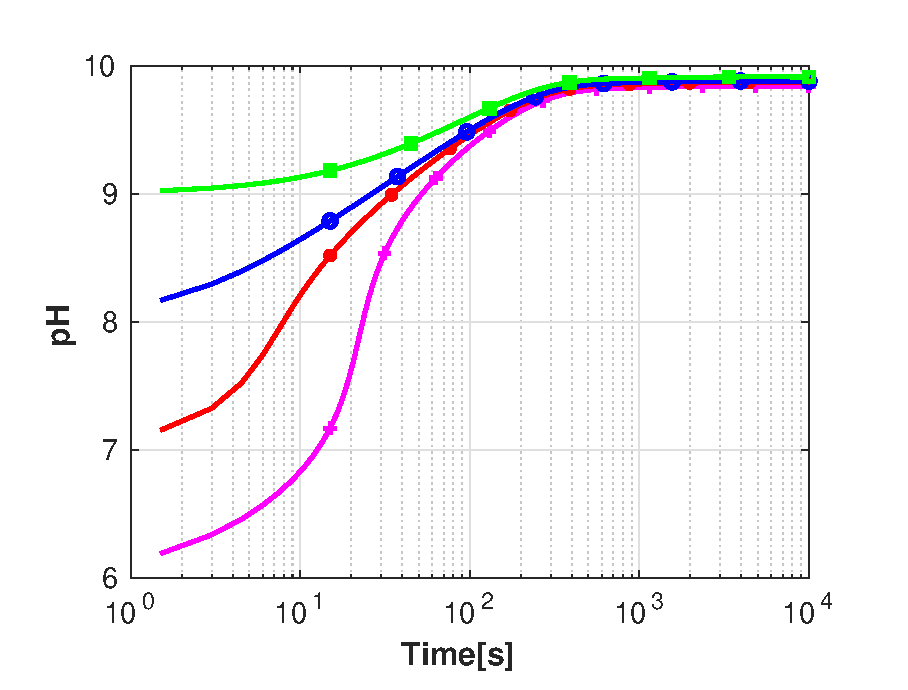
\includegraphics[width=\textwidth]{PICTURES/without_pH_pH.eps}
        \caption{\small Change in pH}
        \label{fig:withoutpHpH}
    \end{subfigure}%
        \hfill
    \begin{subfigure}{.5\linewidth}
            \centering
        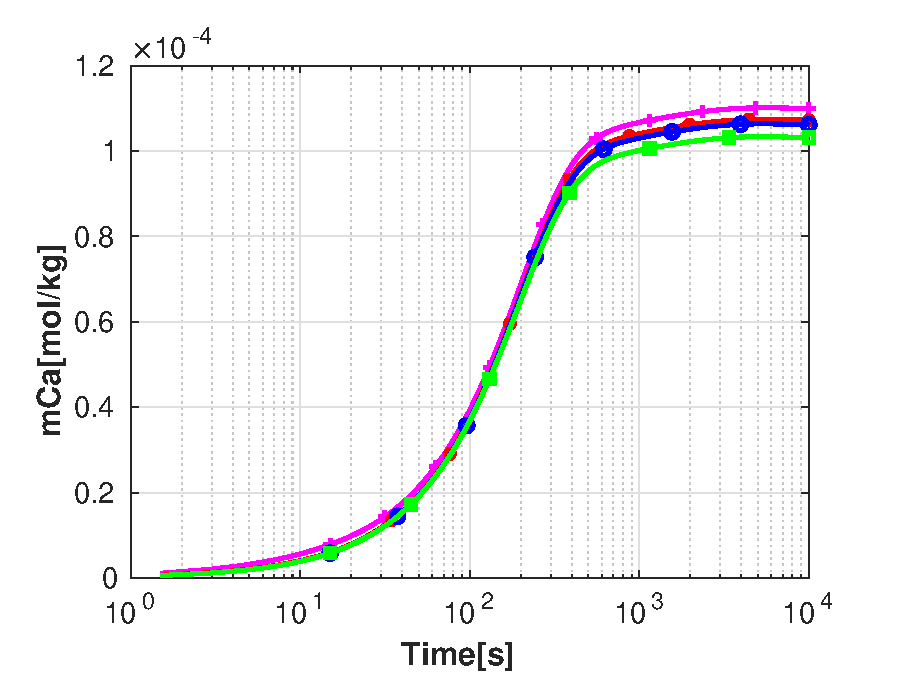
\includegraphics[width=\textwidth]{PICTURES/without_pH_mCa.eps}
        \caption{\small Change in molality of calcium (mCa)}
        \label{fig:withoutpHmCa}
    \end{subfigure}%
    \hfill
    \begin{subfigure}{.5\linewidth}
            \centering
        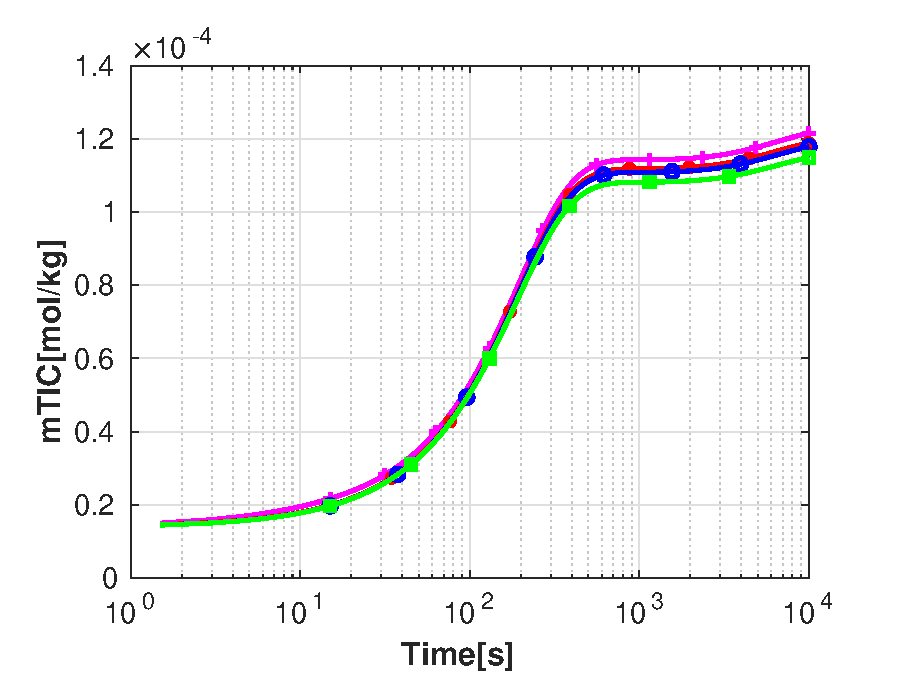
\includegraphics[width=\textwidth]{PICTURES/without_pH_mTIC.eps}
        \caption{\small Change in molality of total inorganic carbon (mTIC)}
        \label{fig:withoutpHmTIC}
    \end{subfigure}%
    \hfill
    \begin{subfigure}{.5\linewidth}
            \centering
        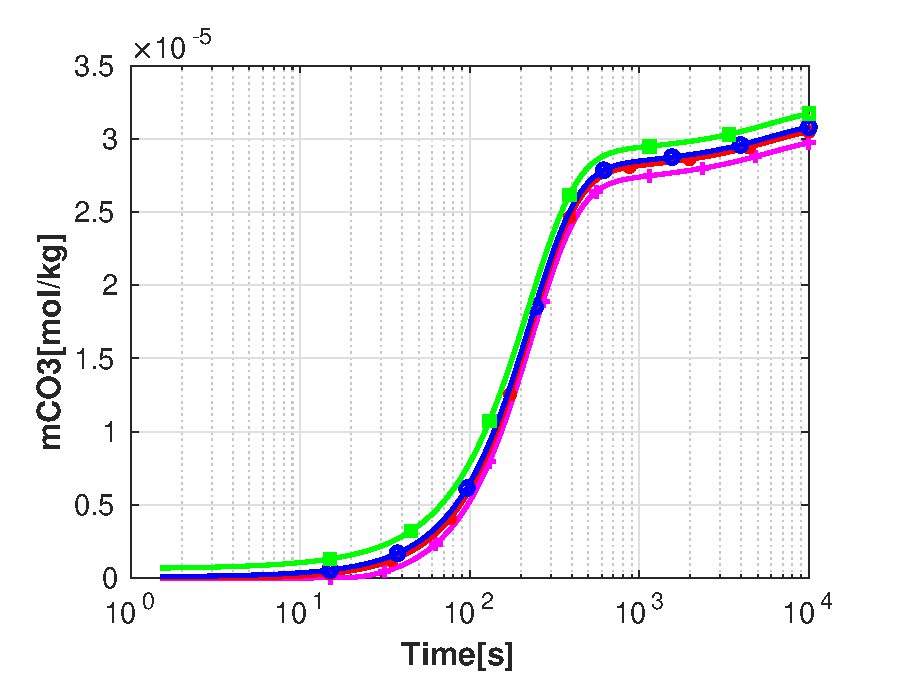
\includegraphics[width=\textwidth]{PICTURES/without_pH_mCO3.eps}
        \caption{\small Change in molality of carbonate (mCO3)}
        \label{fig:withoutpHmCO3}
    \end{subfigure}%
    \hfill
    \begin{subfigure}{.5\linewidth}
            \centering
        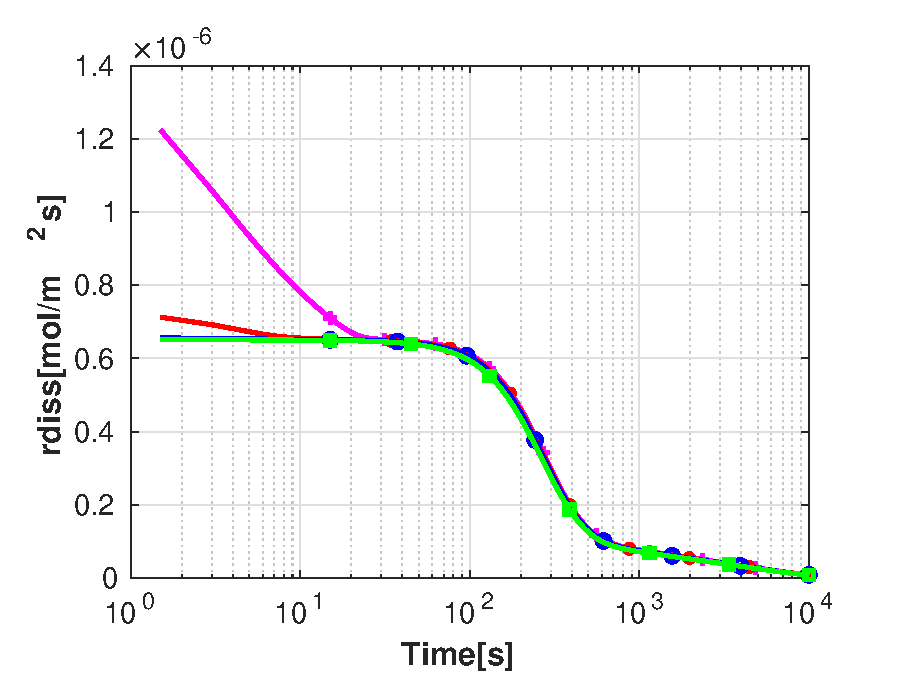
\includegraphics[width=\textwidth]{PICTURES/without_pH_rdiss.eps}
        \caption{\small Change in rate of dissolution of calcite (rdiss)}
        \label{fig:withoutpHrdiss}
    \end{subfigure}%
  \hfill
  \begin{subfigure}{.5\linewidth}
            \centering
        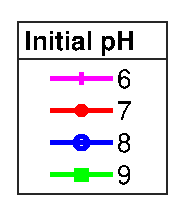
\includegraphics[width=0.25\textwidth]{PICTURES/with_pH_legend.eps}
        \caption{\small Legend}
        \label{fig:withoutpHlegend}
    \end{subfigure}%
    \caption [\DuMuX results for different initial pH in a closed system.] {\textbf{\DuMuX results for different initial pH in a closed system.} \small Time series plot for pH (\Cref{fig:withoutpHpH}), 
    molality of calcium (\Cref{fig:withoutpHmCa}), 
    molality of total inorganic carbon (\Cref{fig:withoutpHmTIC}), molality of carbonate (\Cref{fig:withoutpHmCO3}) 
    and rate of dissolution of calcite (\Cref{fig:withoutpHrdiss}).}
    
    \label{fig:comparisionWithoutDiffInitialpH}
\end{figure}

As we know from \ref{ssec:timeSeriesOpen}, the rate of calcite dissolution and concentration of primary variables 
does not closely depend on the initial pH. Since we had different initial pH of the karst water, the pH and rate of 
dissolution plots (\Cref{fig:withoutpHpH,fig:withoutpHrdiss}) look out of sync at the beginning, just 
like \Cref{fig:pHpH,fig:pHrdiss} but quickly adapts to identical values. 
Unlike in an open system, carbonic acid -- fuel for calcite dissolution -- in a closed system does not get replenished since 
the boundaries are closed to the external environment. As the dissolution proceeds due to the initial concentration 
of TIC present in the water, carbonic acid gets depleted and slowly but surely the rate of calcite dissolution comes to naught (\Cref{fig:withoutpHrdiss}). \\

Carbonic acid near the vicinity of the wall is used up for calcite dissolution. Carbonic acid farther away from the wall reaches the wall by 
diffusion, the only transport mechanism in a closed system. Because of the diffusion, it takes substantial time for 
the rate of calcite dissolution to cease as shown in (\Cref{fig:withoutpHrdiss}). Consequently, the rate of increase in the concentration of TIC and carbonate 
is gradually decreasing and it stabilizes when the dissolution eventually ceases as shown in \Cref{fig:withoutpHmTIC,fig:withoutpHmCO3}.


\section{\MATLAB Simulation results: Closed system}
The scenario we had in \DuMuX for a closed system, where diffusion would mix all the components in water throughout the domain, 
had multiple cells, but in \MATLAB the domain only had one cell which causes the components in the water to mix instantly. \\

\begin{figure}[!h]
        \centering
    \begin{subfigure}{.5\linewidth}
        \centering
        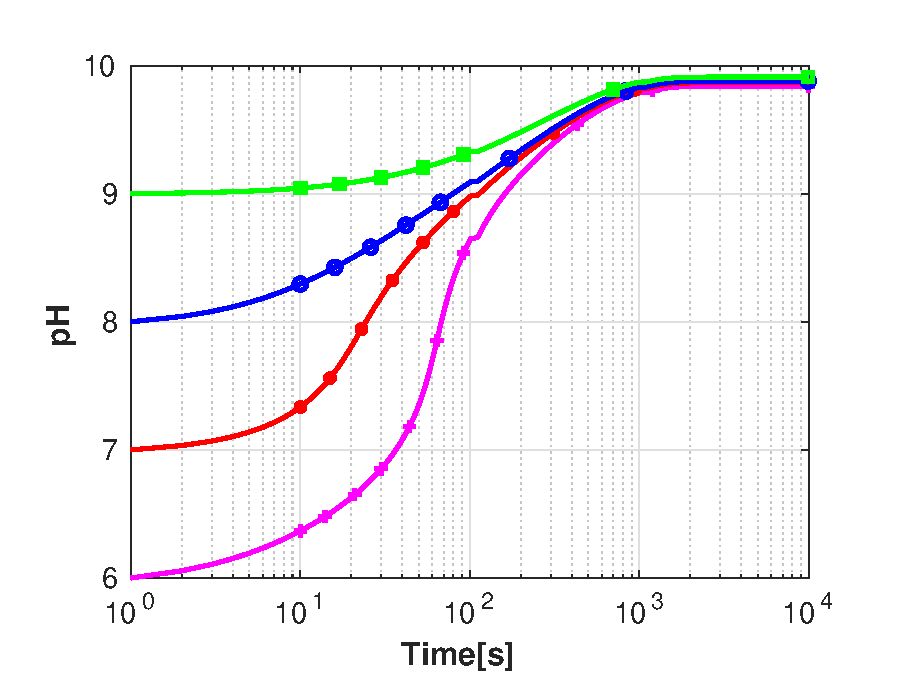
\includegraphics[width=\textwidth]{PICTURES/without_vel_pH.eps}
        \caption{\small Change in pH}
        \label{fig:withoutvelpH}       % Give a unique label
    \end{subfigure}%
        \hfill
        % here was an empty line which caused that the plots where not next
        % to each other but on top of each other
    \begin{subfigure}{.5\linewidth}
        \centering
        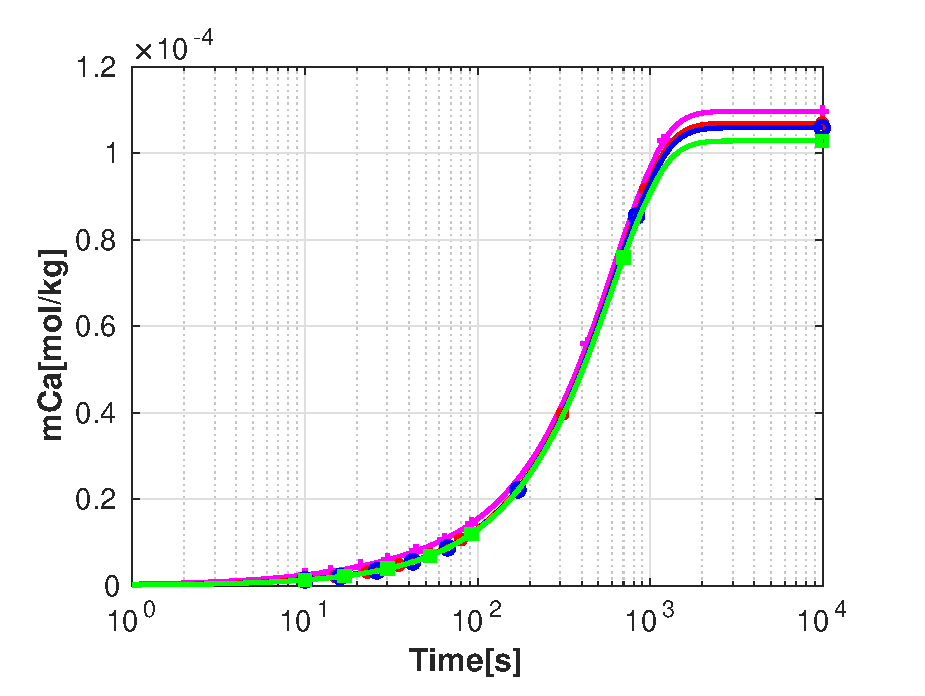
\includegraphics[width=\textwidth]{PICTURES/without_vel_mCa.eps}
        \caption{\small Change in molality of calcium (mCa)}
        \label{fig:withoutvelmCa}       % Give a unique label
    \end{subfigure}%
        \hfill
    \begin{subfigure}{.5\linewidth}
        \centering
        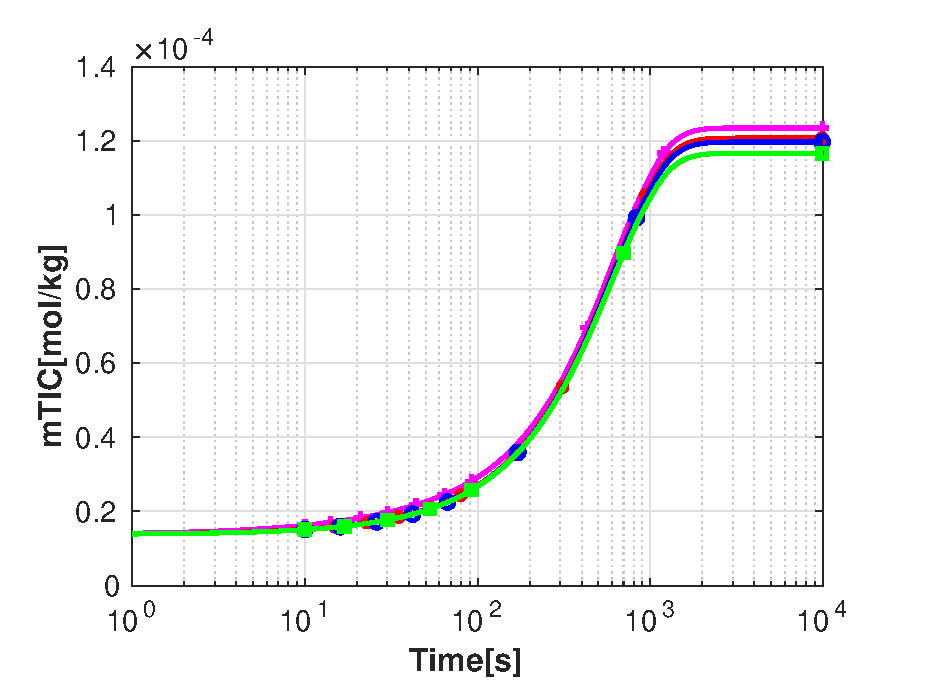
\includegraphics[width=\textwidth]{PICTURES/without_vel_mTIC.eps}
        \caption{\small Change in molality of total inorganic carbon (mTIC)}
        \label{fig:withoutvelmTIC}
    \end{subfigure}%
    \hfill
    \begin{subfigure}{.5\linewidth}
        \centering
        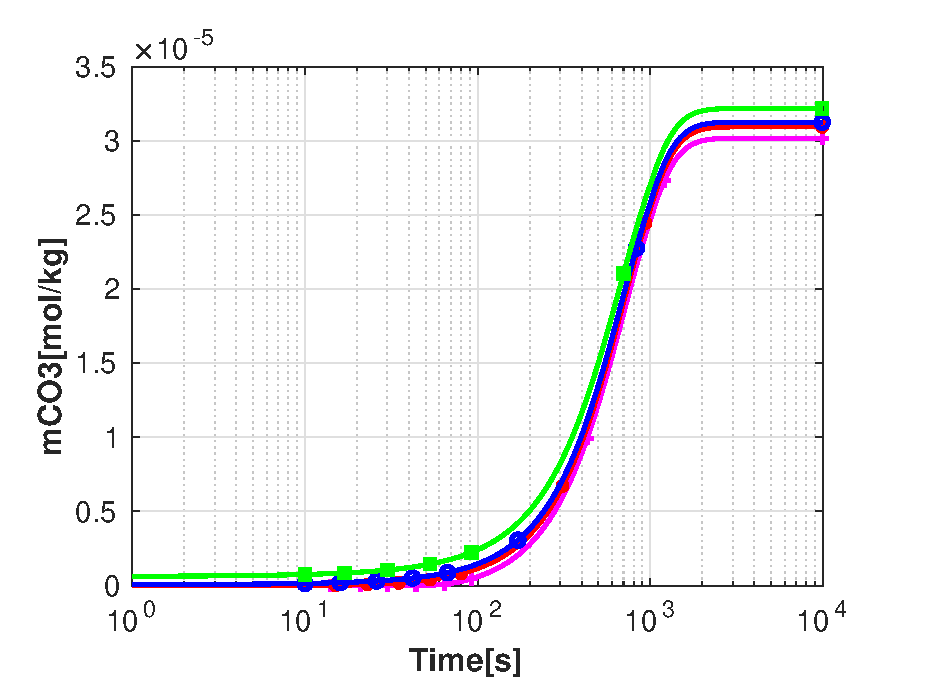
\includegraphics[width=\textwidth]{PICTURES/without_vel_mCO3.eps}
        \caption{\small Change in molality of carbonate (mCO3)}
        \label{fig:withoutvelmCO3}
    \end{subfigure}%
    \hfill
    \begin{subfigure}{.5\linewidth}
        \centering
        \includegraphics[width=\textwidth]{PICTURES/without_vel_rdiss.eps}
        \caption{\small Change in rate of dissolution of calcite (rdiss)}
        \label{fig:withoutvelrdiss}
    \end{subfigure}%
    \hfill
    \begin{subfigure}{.5\linewidth}
        \centering
        \includegraphics[width=0.25\textwidth]{PICTURES/with_pH_legend.eps}
        \caption{\small Legend}
        \label{fig:withoutvellegend}
    \end{subfigure}%
     \caption [\MATLAB results for different initial pH in a closed system.] {\textbf{\MATLAB results for different initial pH in a closed system.} 
     \small Time series plot for pH (\Cref{fig:withoutvelpH}), molality of calcium (\Cref{fig:withoutvelmCa}), 
     molality of total inorganic carbon (\Cref{fig:withoutvelmTIC}), molality of carbonate (\Cref{fig:withoutvelmCO3}) 
     and rate of dissolution of calcite (\Cref{fig:withoutvelrdiss}).}
     \label{fig:MATLABcomparisionDiffInitialpH}
\end{figure}

\MATLAB results (\Cref{fig:MATLABcomparisionDiffInitialpH}) look very similar to the \DuMuX results (\Cref{fig:comparisionWithoutDiffInitialpH}) 
for a closed system with varying initial pH as described in \Cref{ssec:diffinitialpHnoflow}. Instant mixing of components throughout the domain 
in the \MATLAB model results in a faster approach to steady-state. In \DuMuX it was diffusion that mixed the components throughout the domain. \\

The higher the initial pH, the lower is the initial rate of calcite dissolution, since the basic solution slows down the calcite dissociation 
as shown in \Cref{fig:withoutvelpH,fig:withoutvelrdiss}.

\section{Comparison: \DuMuX and \MATLAB} \label{sec:dvm}
Identical initial and boundary conditions and a domain with just one cell of size [5mm$\times$15mm] were set in both \MATLAB and \DuMuX 
to carry out the comparison. The initial pH of karst water and the reactive area/batch volume were varied to compare the results. 
For a 2D domain, a reactive area is defined as the length of the reactive wall and a batch volume is the area of the cell where dissolution occurs. 
We assumed four different initial pH (6, 7, 8, and 9), and three different reactive area/batch 
volume (5mm/5\ce{mm^2}, 15mm/75\ce{mm^2}, and 30mm/300\ce{mm^2}) for simulation runs. We set the initial concentration of TIC 
throughout the domain to 2.5e-7 [mol\_\ce{TIC}/mol\_\ce{H2O}], 
an assumed value. \Cref{fig:ClosedSystem} shows the model domain and boundary conditions set in \MATLAB and \DuMuX for this scenario. \\

\begin{table}[ht]
\small\addtolength{\tabcolsep}{-12pt}
\centering
\caption [\DuMuX and \MATLAB comparison table.] {\textbf{\DuMuX and \MATLAB comparison table.} \small The table lists steady-state time, pH, molality of calcium (mCa), 
molality of total inorganic carbon (mTIC) and molality of carbonate (mCO3) for a closed system of size 
[15mm$\times$5mm] with varying initial pH and reactive area/batch volume.}
\begin{tabular}{|c|c|c|c|c|c|c|c|c|c|c|c|c|}
    \hline
    \thead{Initial \\pH} & \thead{Reactive \\area} & \thead{Batch \\Volume} & \multicolumn{5}{c|}{\thead{Steady-state \MATLAB}} & 
    \multicolumn{5}{c|}{\thead{Steady-state \DuMuX}} \\
    \cline{4-13}
    & & & \thead{time} & \thead{pH} & \thead{mCa}      & \thead{mTIC}     & \thead{mCO3}     & \thead{time} & \thead{pH} & \thead{mCa}      
    & \thead{mTIC}     & \thead{mCO3}\\
    & mm & \ce{mm^2} &  [s]  & [-] & [mol/kg] & [mol/kg] & [mol/kg] & [s] & [-]   & [mol/kg] & [mol/kg] & [mol/kg]\\
    \hline
    % initial pH   Reactive area Batch Volume time pH mCa mTIC mCO3 time pH mCa mTIC mCO3
      & 5  & 5   & 321  & 9.83 & 1.09e-4 & 1.23e-4 & 3.01e-5 & 321 & 9.83 & 1.09e-4 & 1.23e-4 & 3.01e-5 \\
    6 & 15 & 75  & 1601 & 9.83 & 1.09e-4 & 1.23e-4 & 3.01e-5 & 1596 & 9.83 & 1.09e-4 & 1.23e-4 & 3.01e-5 \\
      & 30 & 300 & 3201 & 9.83 & 1.09e-4 & 1.23e-4 & 3.01e-5 & 3190 & 9.83 & 1.09e-4 & 1.23e-4 & 3.01e-5 \\
    \hline
      & 5  & 5   & 331  & 9.86 & 1.06e-4 & 1.20e-4 & 3.09e-5 & 338  & 9.86 & 1.06e-4 & 1.20e-4 & 3.09e-5 \\
    7 & 15 & 75  & 1701 & 9.86 & 1.06e-4 & 1.20e-4 & 3.09e-5 & 1679 & 9.86 & 1.06e-4 & 1.20e-4 & 3.09e-5 \\
      & 30 & 300 & 3301 & 9.86 & 1.06e-4 & 1.20e-4 & 3.09e-5 & 3357 & 9.86 & 1.06e-4 & 1.20e-4 & 3.09e-5 \\
    \hline
      & 5  & 5   & 321  & 9.87 & 1.05e-4 & 1.19e-4 & 3.12e-5 & 324  & 9.87 & 1.05e-4 & 1.19e-4 & 3.12e-5 \\
    8 & 15 & 75  & 1701 & 9.87 & 1.05e-4 & 1.19e-4 & 3.12e-5 & 1610 & 9.87 & 1.05e-4 & 1.19e-4 & 3.12e-5 \\
      & 30 & 300 & 3201 & 9.87 & 1.05e-4 & 1.19e-4 & 3.12e-5 & 3219 & 9.87 & 1.05e-4 & 1.19e-4 & 3.12e-5 \\
    \hline
      & 5  & 5   & 611  & 9.91 & 1.02e-4 & 1.16e-4 & 3.21e-5 & 294  & 9.90 & 1.02e-4 & 1.16e-4 & 3.21e-5 \\
    9 & 15 & 75  & 3001 & 9.91 & 1.02e-4 & 1.16e-4 & 3.21e-5 & 1463 & 9.90 & 1.02e-4 & 1.16e-4 & 3.21e-5 \\
      & 30 & 300 & 6101 & 9.91 & 1.02e-4 & 1.16e-4 & 3.21e-5 & 2924 & 9.90 & 1.02e-4 & 1.16e-4 & 3.21e-5 \\
    \hline
\end{tabular}
% \end{adjustbox}
\label{tab:DumuxVsMatlab}
\end{table}

\Cref{tab:DumuxVsMatlab} shows \MATLAB results agree closely with \DuMuX results at the steady-state. A slight disagreement in the steady-state time is 
because of the difference in the time step size between the two models. \\

\begin{figure}[!h]
        \centering
    \begin{subfigure}{.5\linewidth}
            \centering
        \includegraphics[width=\textwidth]{PICTURES/dvm_pH6_pH.eps}
        \caption{\small Change in pH}
        \label{fig:dvmpH6pH}
    \end{subfigure}%
        \hfill
    \begin{subfigure}{.5\linewidth}
            \centering
        \includegraphics[width=\textwidth]{PICTURES/dvm_pH6_mCa.eps}
        \caption{\small Change in molality of calcium (mCa)}
        \label{fig:dvmpH6mCa}
    \end{subfigure}%
    \hfill
    \begin{subfigure}{.5\linewidth}
            \centering
        \includegraphics[width=\textwidth]{PICTURES/dvm_pH6_mTIC.eps}
        \caption{\small Change in molality of total inorganic carbon (mTIC)}
        \label{fig:dvmpH6mTIC}
    \end{subfigure}%
    \hfill
    \begin{subfigure}{.5\linewidth}
            \centering
        \includegraphics[width=\textwidth]{PICTURES/dvm_pH6_mCO3.eps}
        \caption{\small Change in molality of carbonate (mCO3)}
        \label{fig:dvmpH6mCO3}
    \end{subfigure}%
    \hfill
    \begin{subfigure}{.5\linewidth}
            \centering
        \includegraphics[width=\textwidth]{PICTURES/dvm_pH6_rdiss.eps}
        \caption{\small Change in rate of dissolution of calcite (rdiss)}
        \label{fig:dvmpH6rdiss}
    \end{subfigure}%
  \hfill
  \hfill
    \begin{subfigure}{.5\linewidth}
            \centering
        \includegraphics[width=0.85\textwidth]{PICTURES/dvm_pH6_legend.eps}
        \caption{\small Legend}
        \label{fig:dvmpH6legend}
    \end{subfigure}%
    \caption [Comparison: \DuMuX and \MATLAB results for initial pH 6.0 in a closed system.] {\textbf{ Comparison: \DuMuX and \MATLAB 
    results for initial pH 6.0 in a closed system.} \small Time series plot for pH (\Cref{fig:dvmpH6pH}), 
    molality of calcium (\Cref{fig:dvmpH6mCa}), molality of total inorganic carbon (\Cref{fig:dvmpH6mTIC}), 
    molality of carbonate (\Cref{fig:dvmpH6mCO3}) and rate of dissolution of calcite (\Cref{fig:dvmpH6rdiss}).} 
    \label{fig:comparisionDumuxMatlab_pH6.0}
\end{figure}

Time series plot for initial pH 6 (\Cref{fig:comparisionDumuxMatlab_pH6.0}) also shows \MATLAB results agree closely with \DuMuX results. 
Time series plot for initial pH 7, 8 and 9 are presented in \Cref{app:appendixB}.


\endinput